\crefalias{section}{appendix}
\crefalias{subsection}{appendix}

\renewcommand{\thesection}{\Alph{section}}

\begin{appendices}
\section{Additional results for \Cref{chap:anisotropy}}
\subsection{Other projections for $Q^h_s$ and $K^h_s$}
\label{sec:other_projs}

As mentioned in the Discussion (\Cref{sec:anisotropy_discussion}), we reproduce visualizations from \Cref{sec:qk} using different projection choices. Namely, we compute the SVD on $K^h_s$ only in \Cref{fig:proj_qk_heads_K} and \Cref{fig:QK_dir_K}, and on $Q^h_s$ only in \Cref{fig:proj_qk_heads_Q} and \Cref{fig:QK_dir_Q}.

The plots show that not only does the distribution used for the SVD drifts away from the origin along training, but also that the other distribution drifts away from the origin in an opposite direction. In other words, the singular components of each distribution are also relevant to describe the drift of the other distribution. Hence, \Cref{fig:proj_qk_heads_K} and \Cref{fig:proj_qk_heads_Q} support our conclusion that the drift directions of keys and queries are aligned during training.


\begin{figure*}[ht]
    \centering
    \begin{subfigure}[b]{0.24\linewidth}
         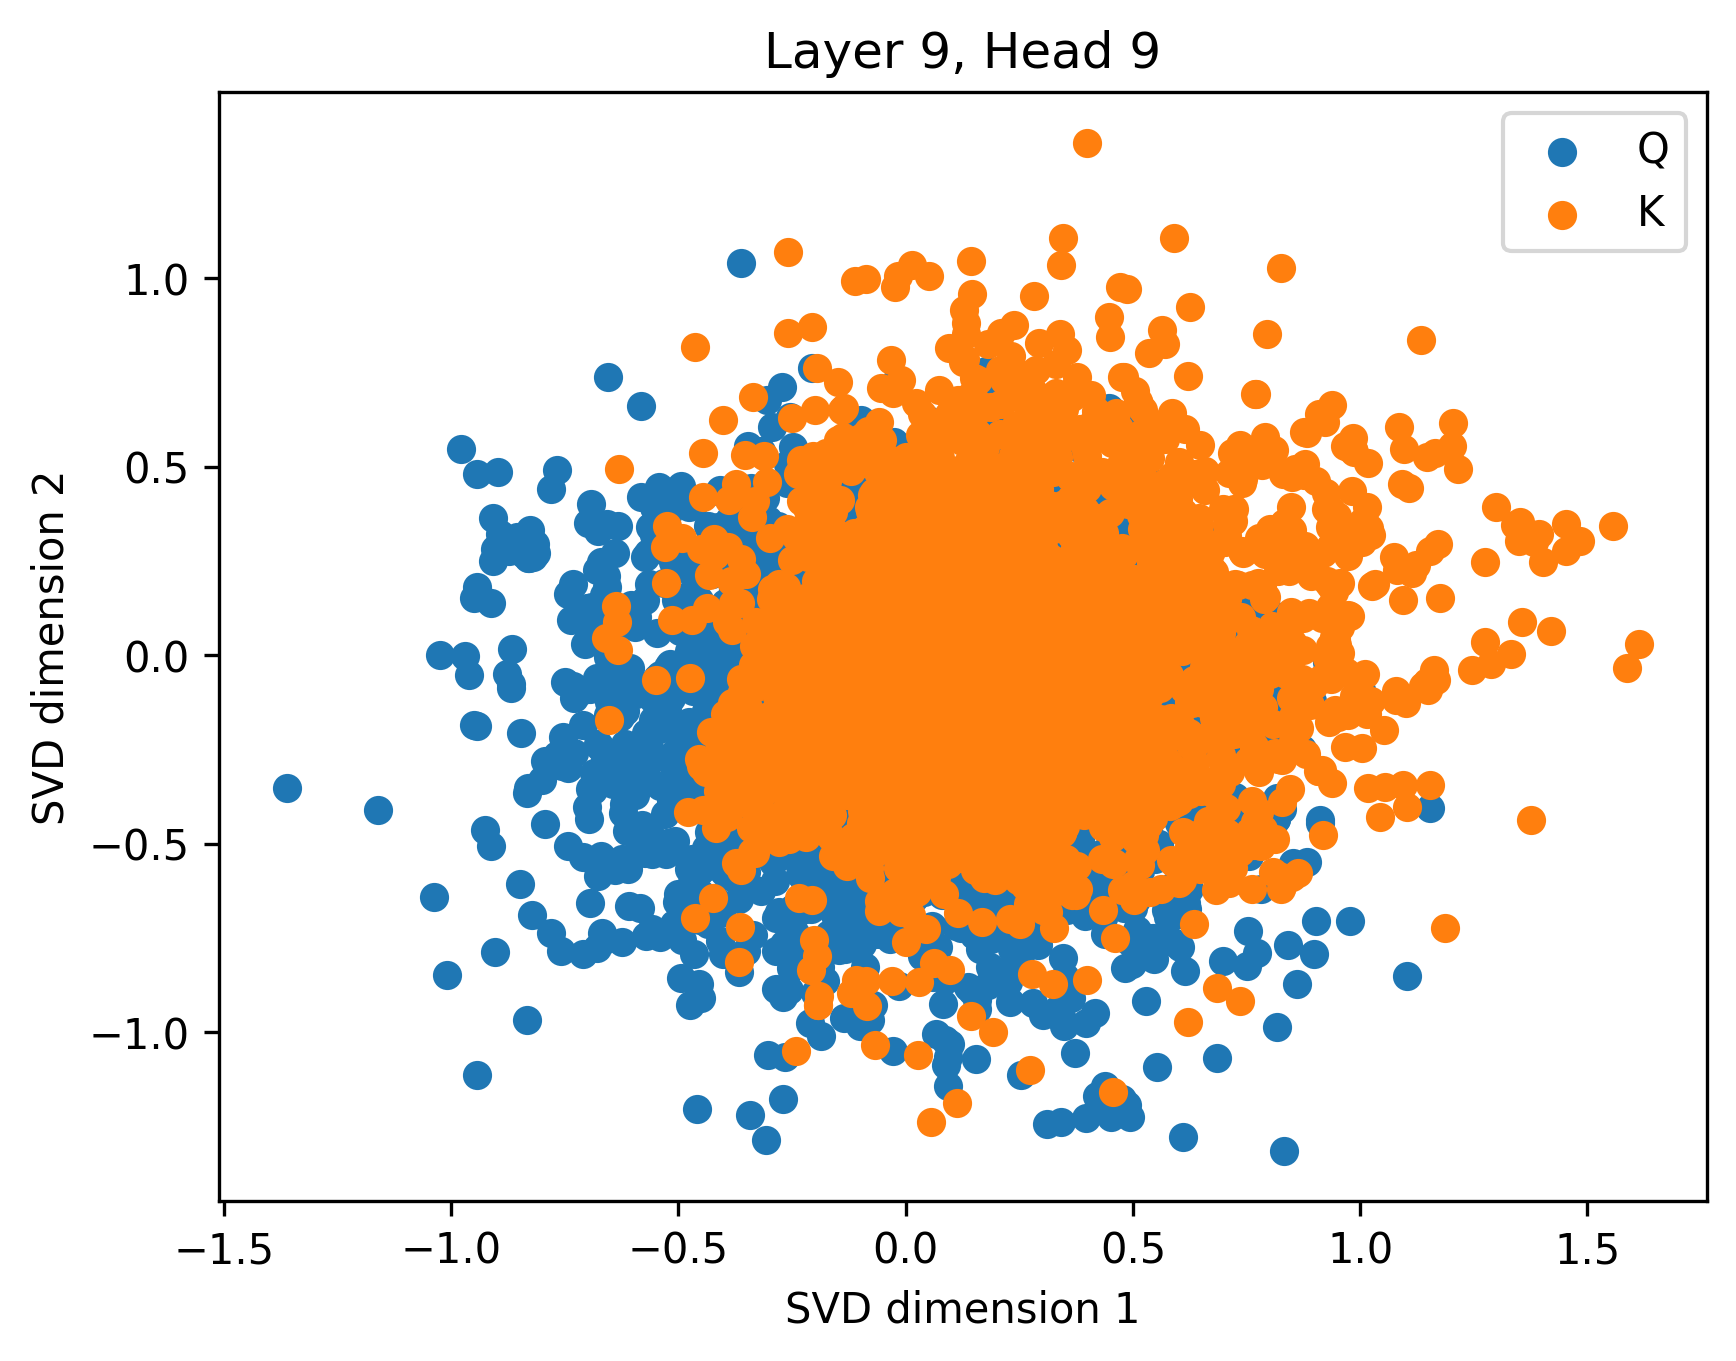
\includegraphics[width=\linewidth]{sources/part_1/anisotropy/imgs/dist_l9h9_s0_K.png}
         \caption{Step 0}
         \label{fig:dist_qk_s0_K}
    \end{subfigure}
    \begin{subfigure}[b]{0.24\linewidth}
         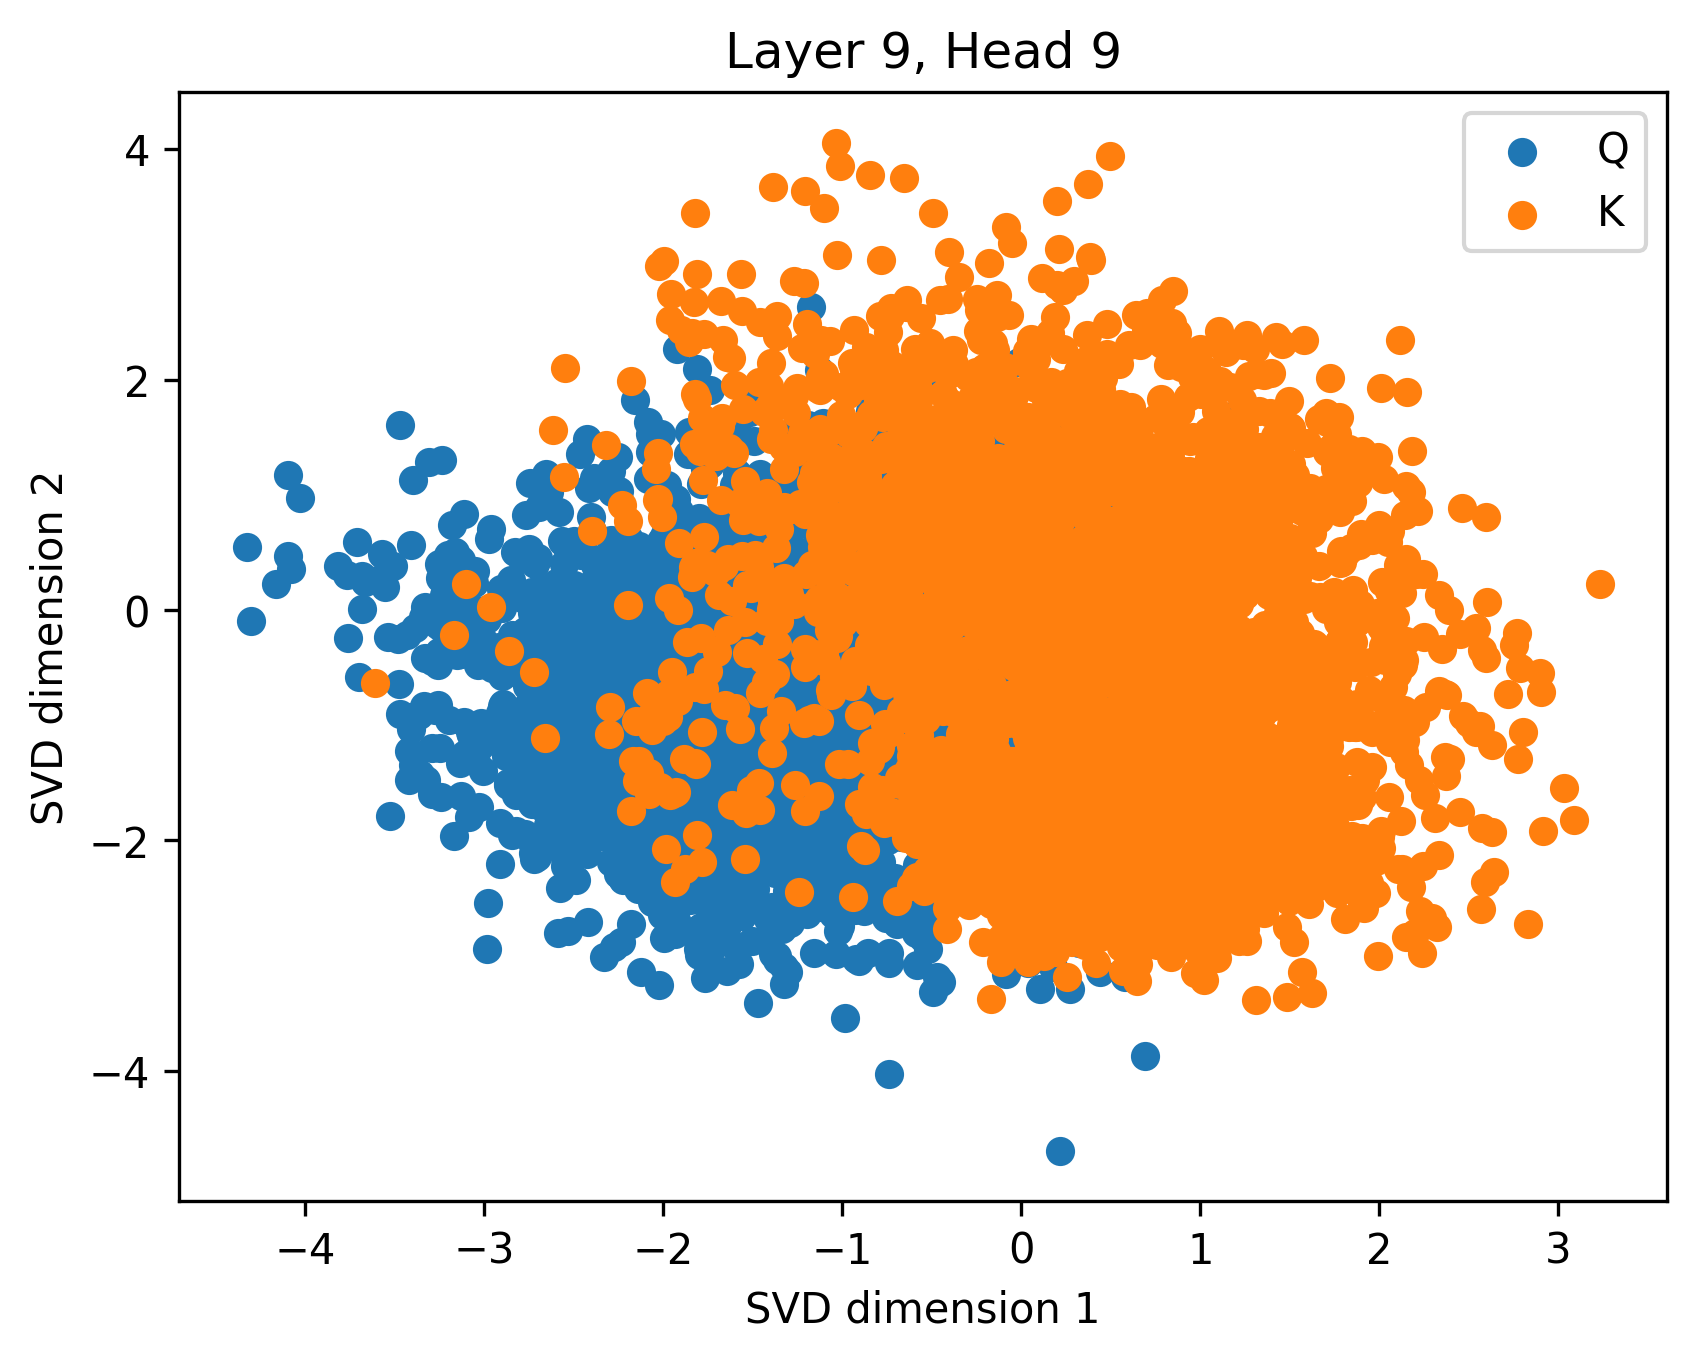
\includegraphics[width=\linewidth]{sources/part_1/anisotropy/imgs/dist_l9h9_s40_K.png}
         \caption{Step 40k}
         \label{fig:dist_qk_s40_K}
    \end{subfigure}
    \begin{subfigure}[b]{0.24\linewidth}
         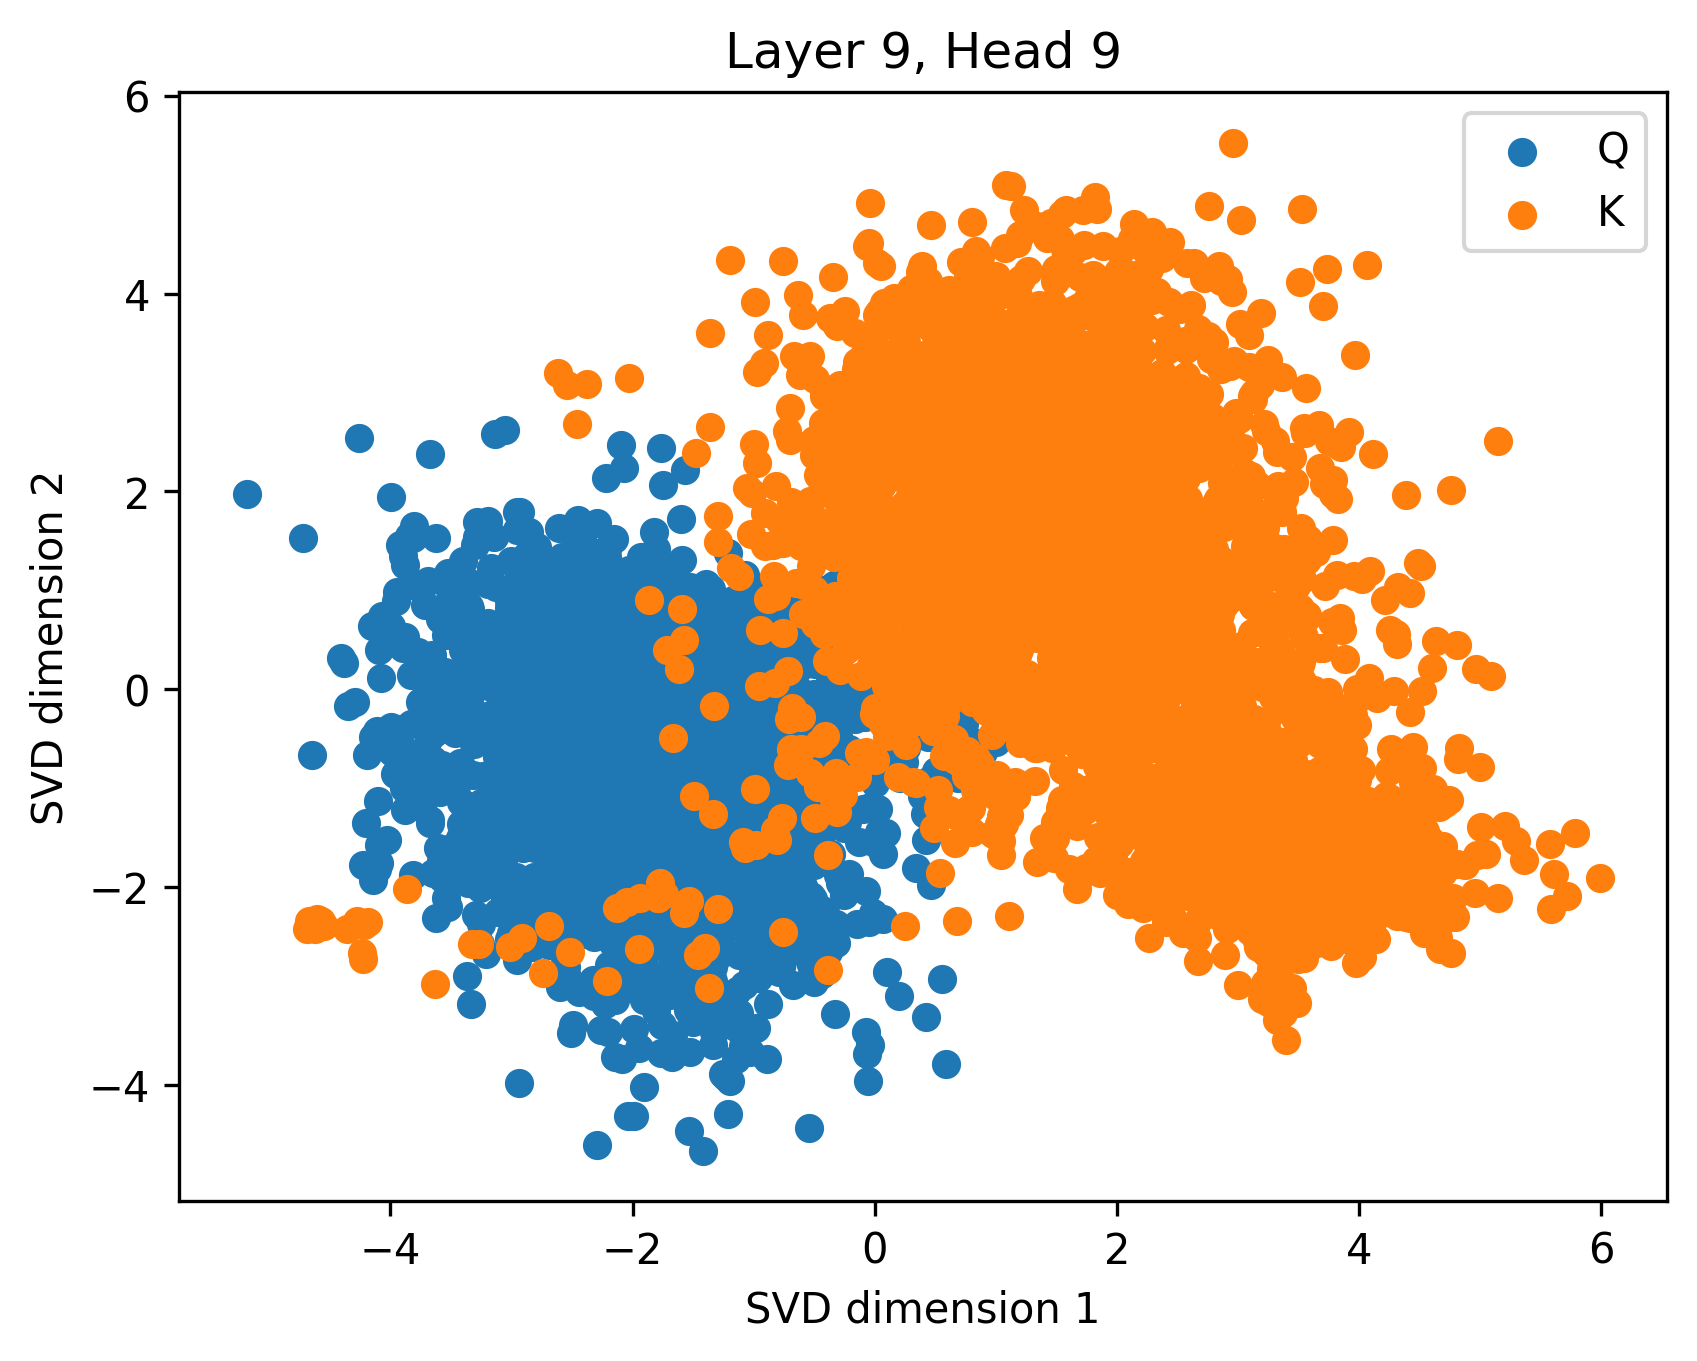
\includegraphics[width=\linewidth]{sources/part_1/anisotropy/imgs/dist_l9h9_s200_K.png}
         \caption{Step 200k}
         \label{fig:dist_qk_s200_K}
    \end{subfigure}
    \begin{subfigure}[b]{0.24\linewidth}
         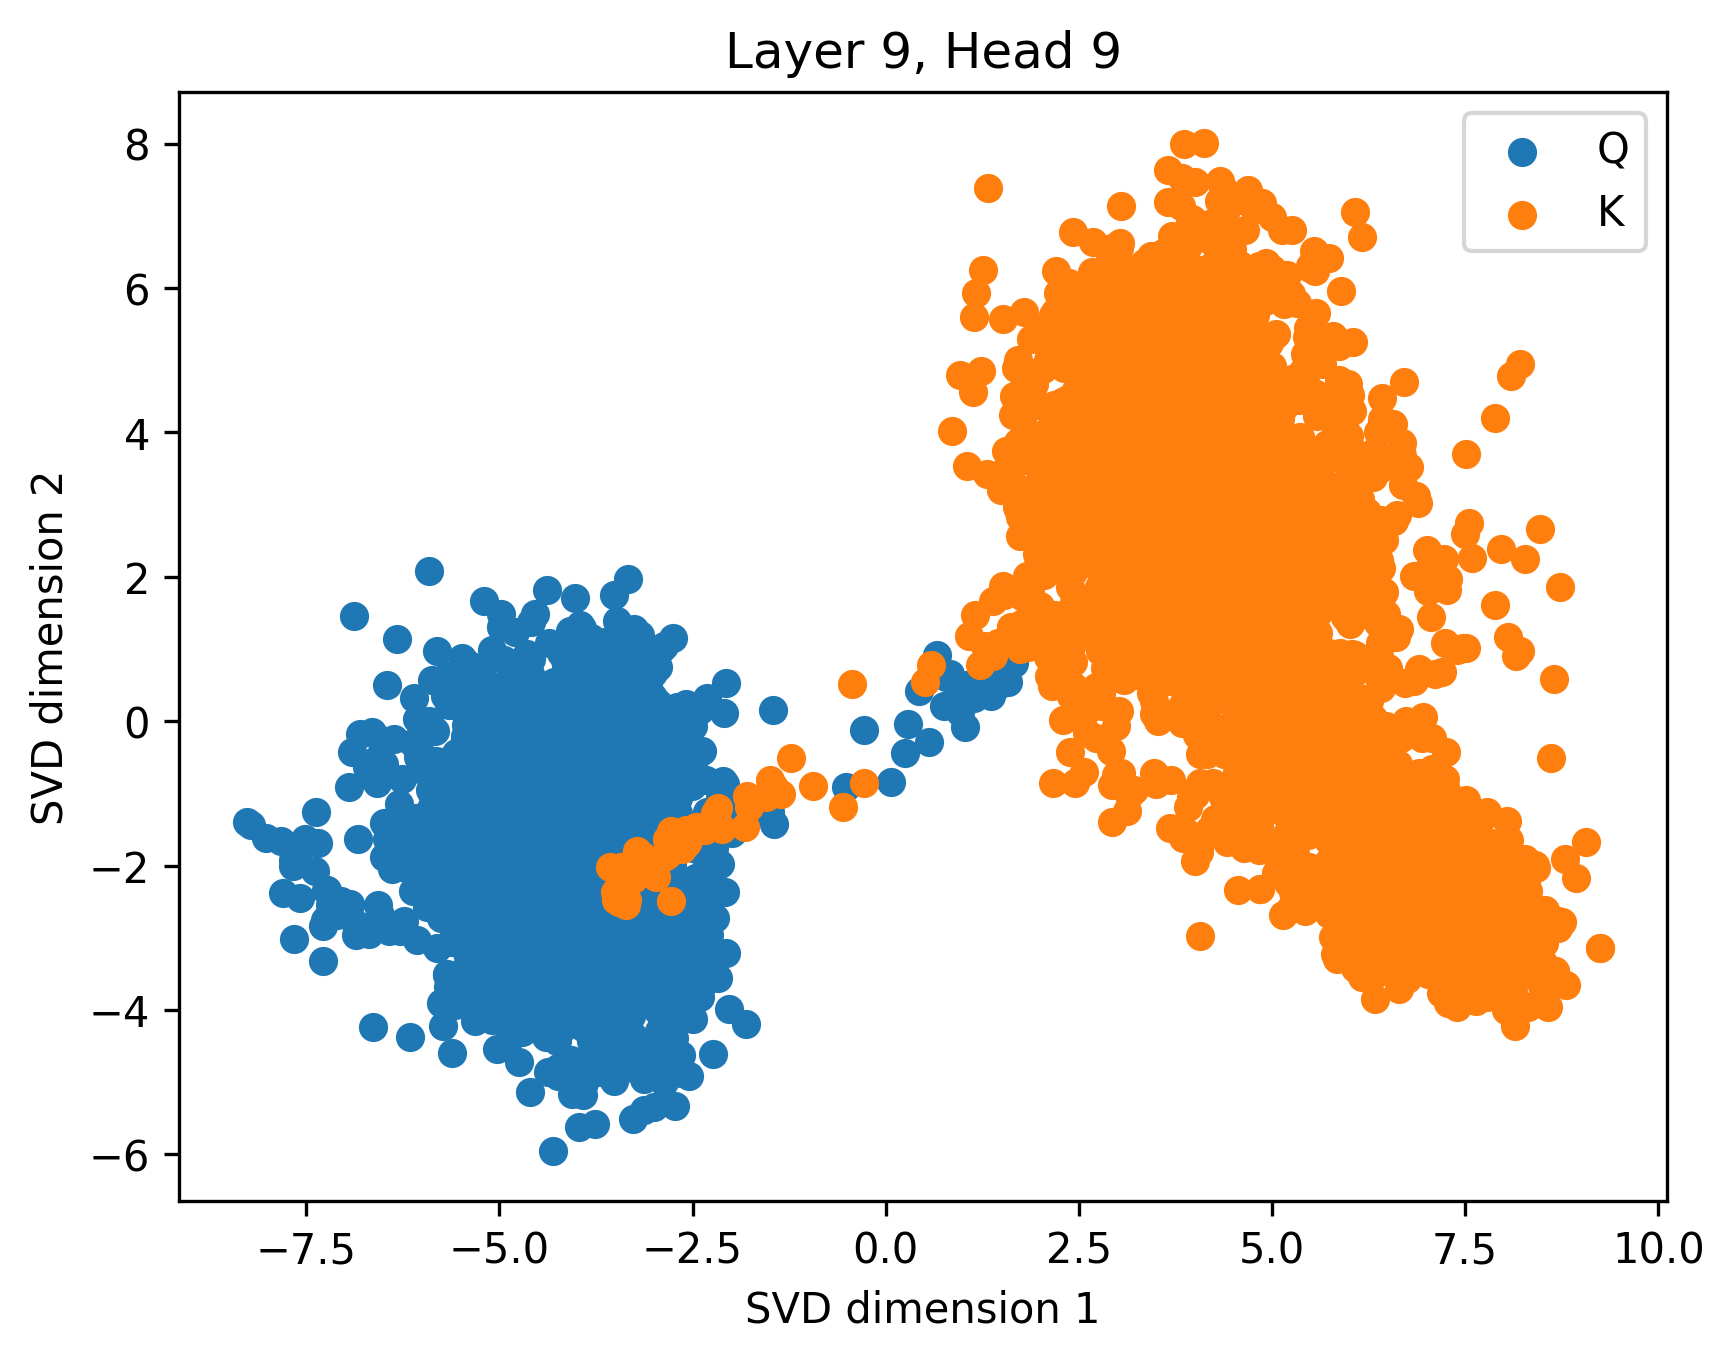
\includegraphics[width=\linewidth]{sources/part_1/anisotropy/imgs/dist_l9h9_s2000_K.png}
         \caption{Step 2M (final)}
         \label{fig:dist_qk_s2M_K}
    \end{subfigure}
    \caption{Evolution of $Q^h_s$ and $K^h_s$ distributions along training. Vectors are projected using the SVD computed on $K^h_s$.}
    \label{fig:proj_qk_heads_K}
\end{figure*}

\begin{figure*}[ht]
    \centering
    \begin{subfigure}[b]{0.24\linewidth}
         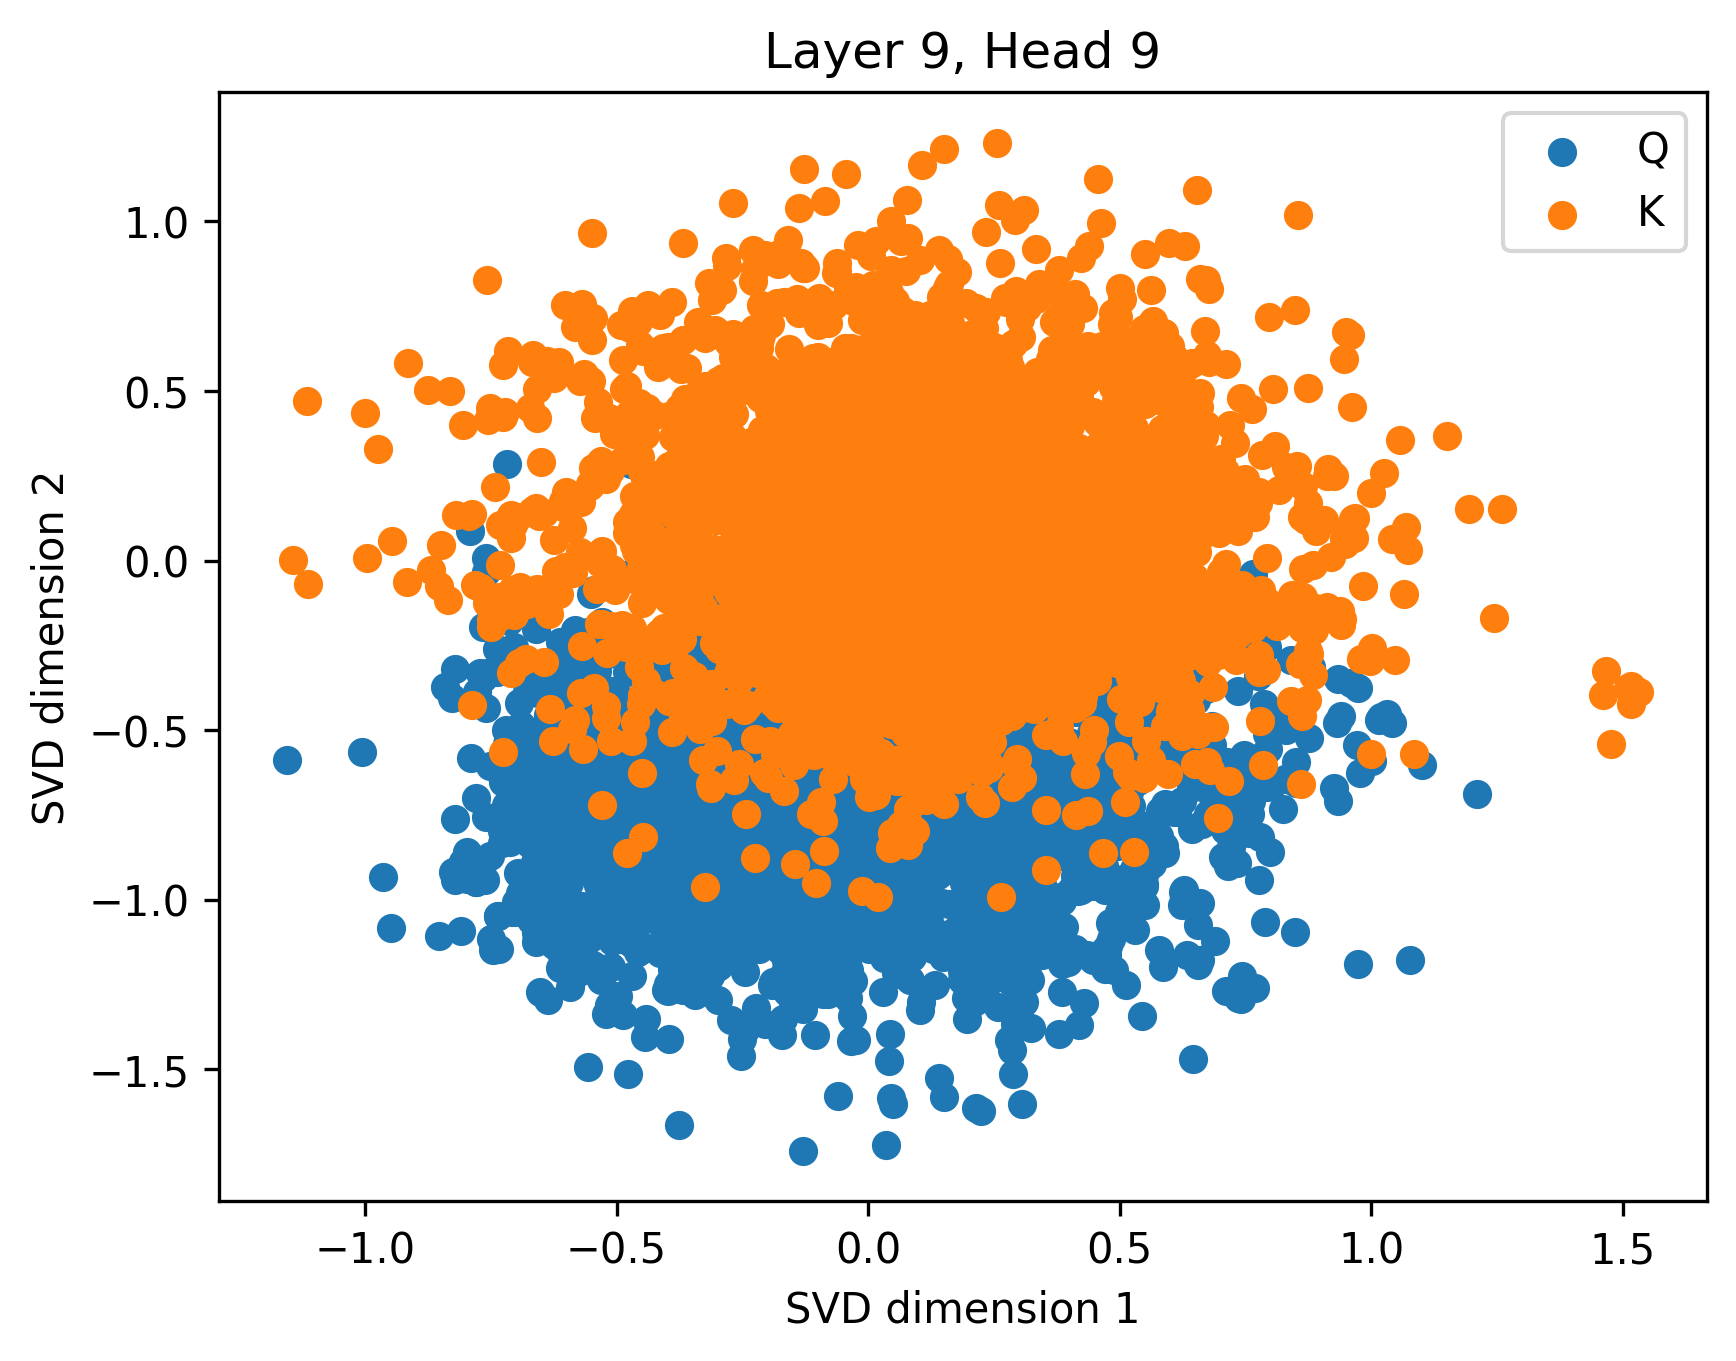
\includegraphics[width=\linewidth]{sources/part_1/anisotropy/imgs/dist_l9h9_s0_Q.png}
         \caption{Step 0}
         \label{fig:dist_qk_s0_Q}
    \end{subfigure}
    \begin{subfigure}[b]{0.24\linewidth}
         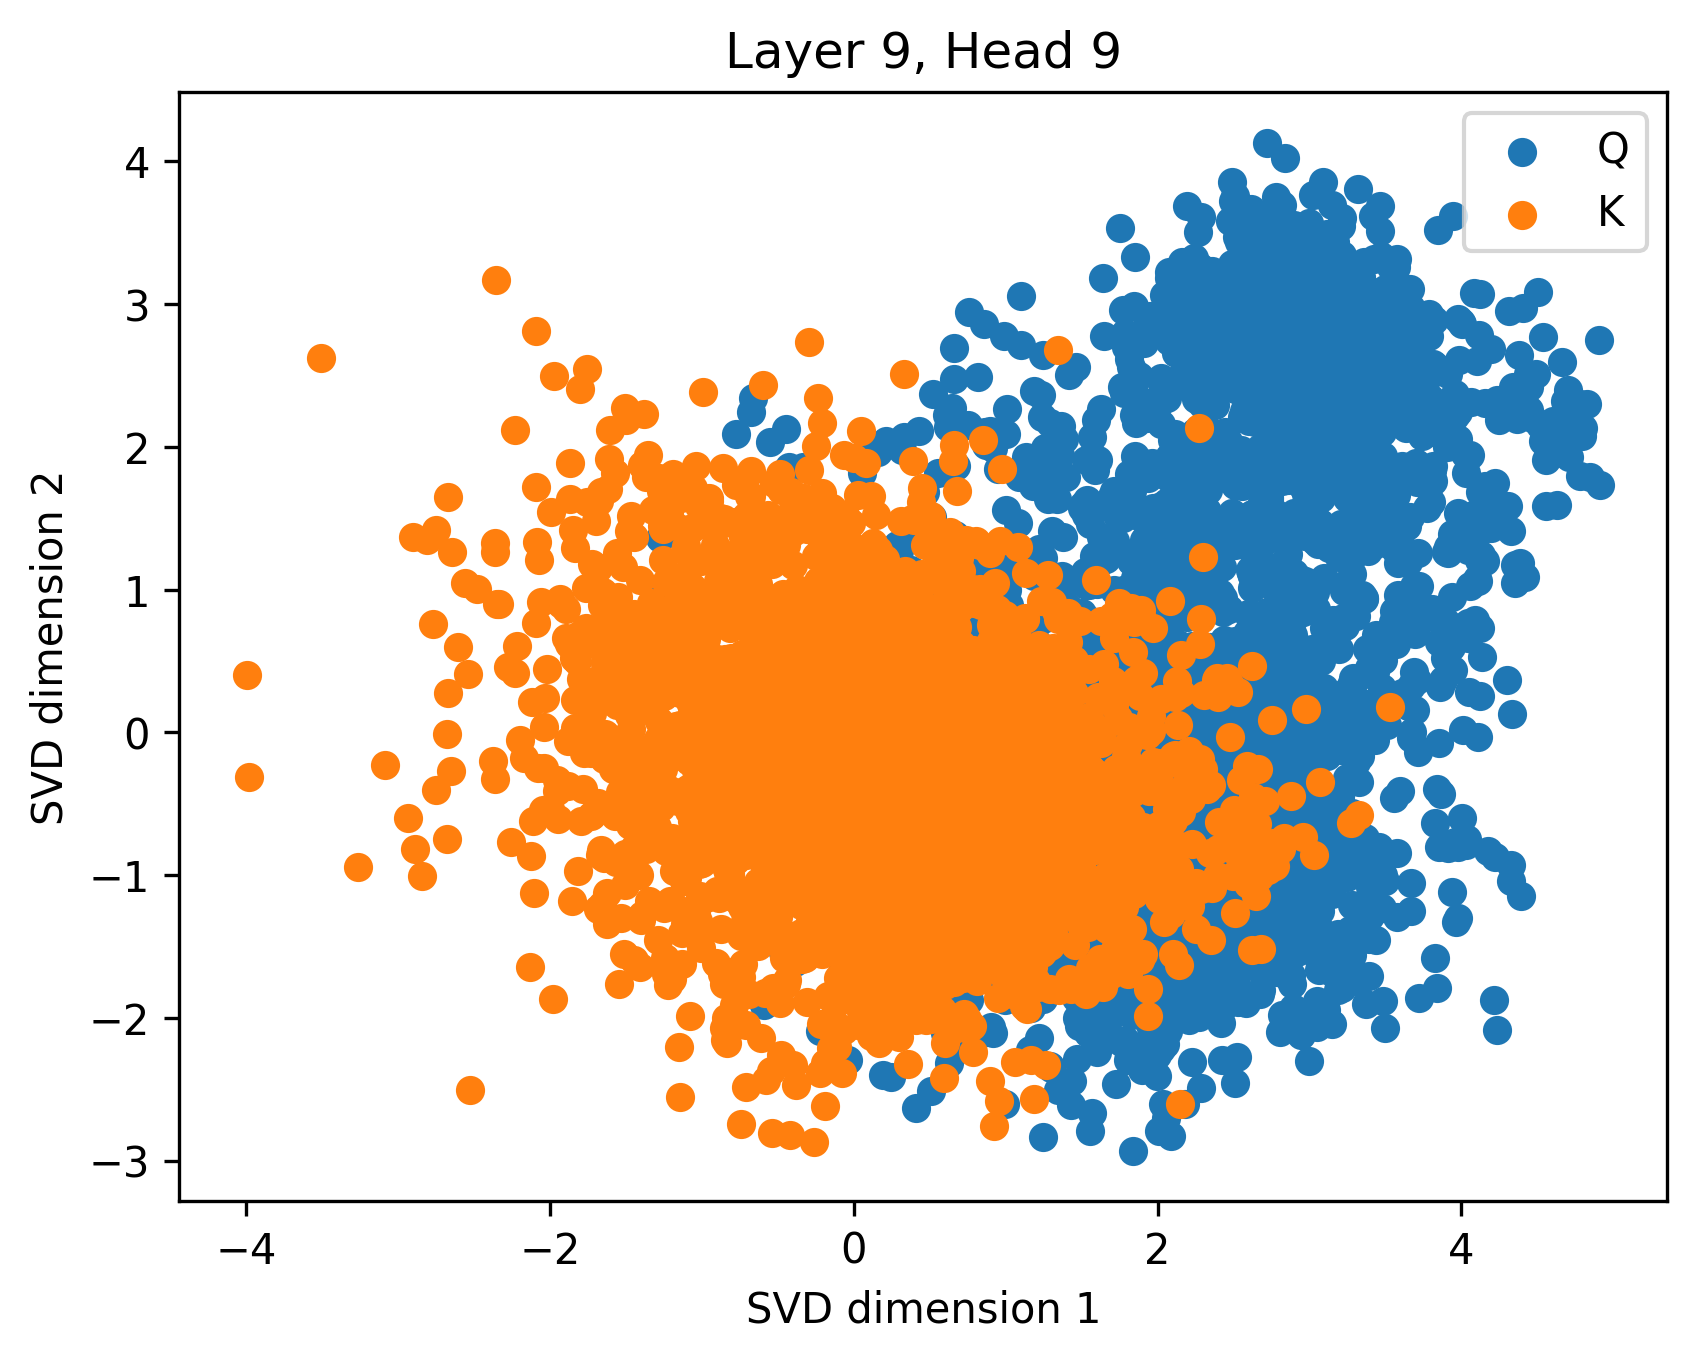
\includegraphics[width=\linewidth]{sources/part_1/anisotropy/imgs/dist_l9h9_s40_Q.png}
         \caption{Step 40k}
         \label{fig:dist_qk_s40_Q}
    \end{subfigure}
    \begin{subfigure}[b]{0.24\linewidth}
         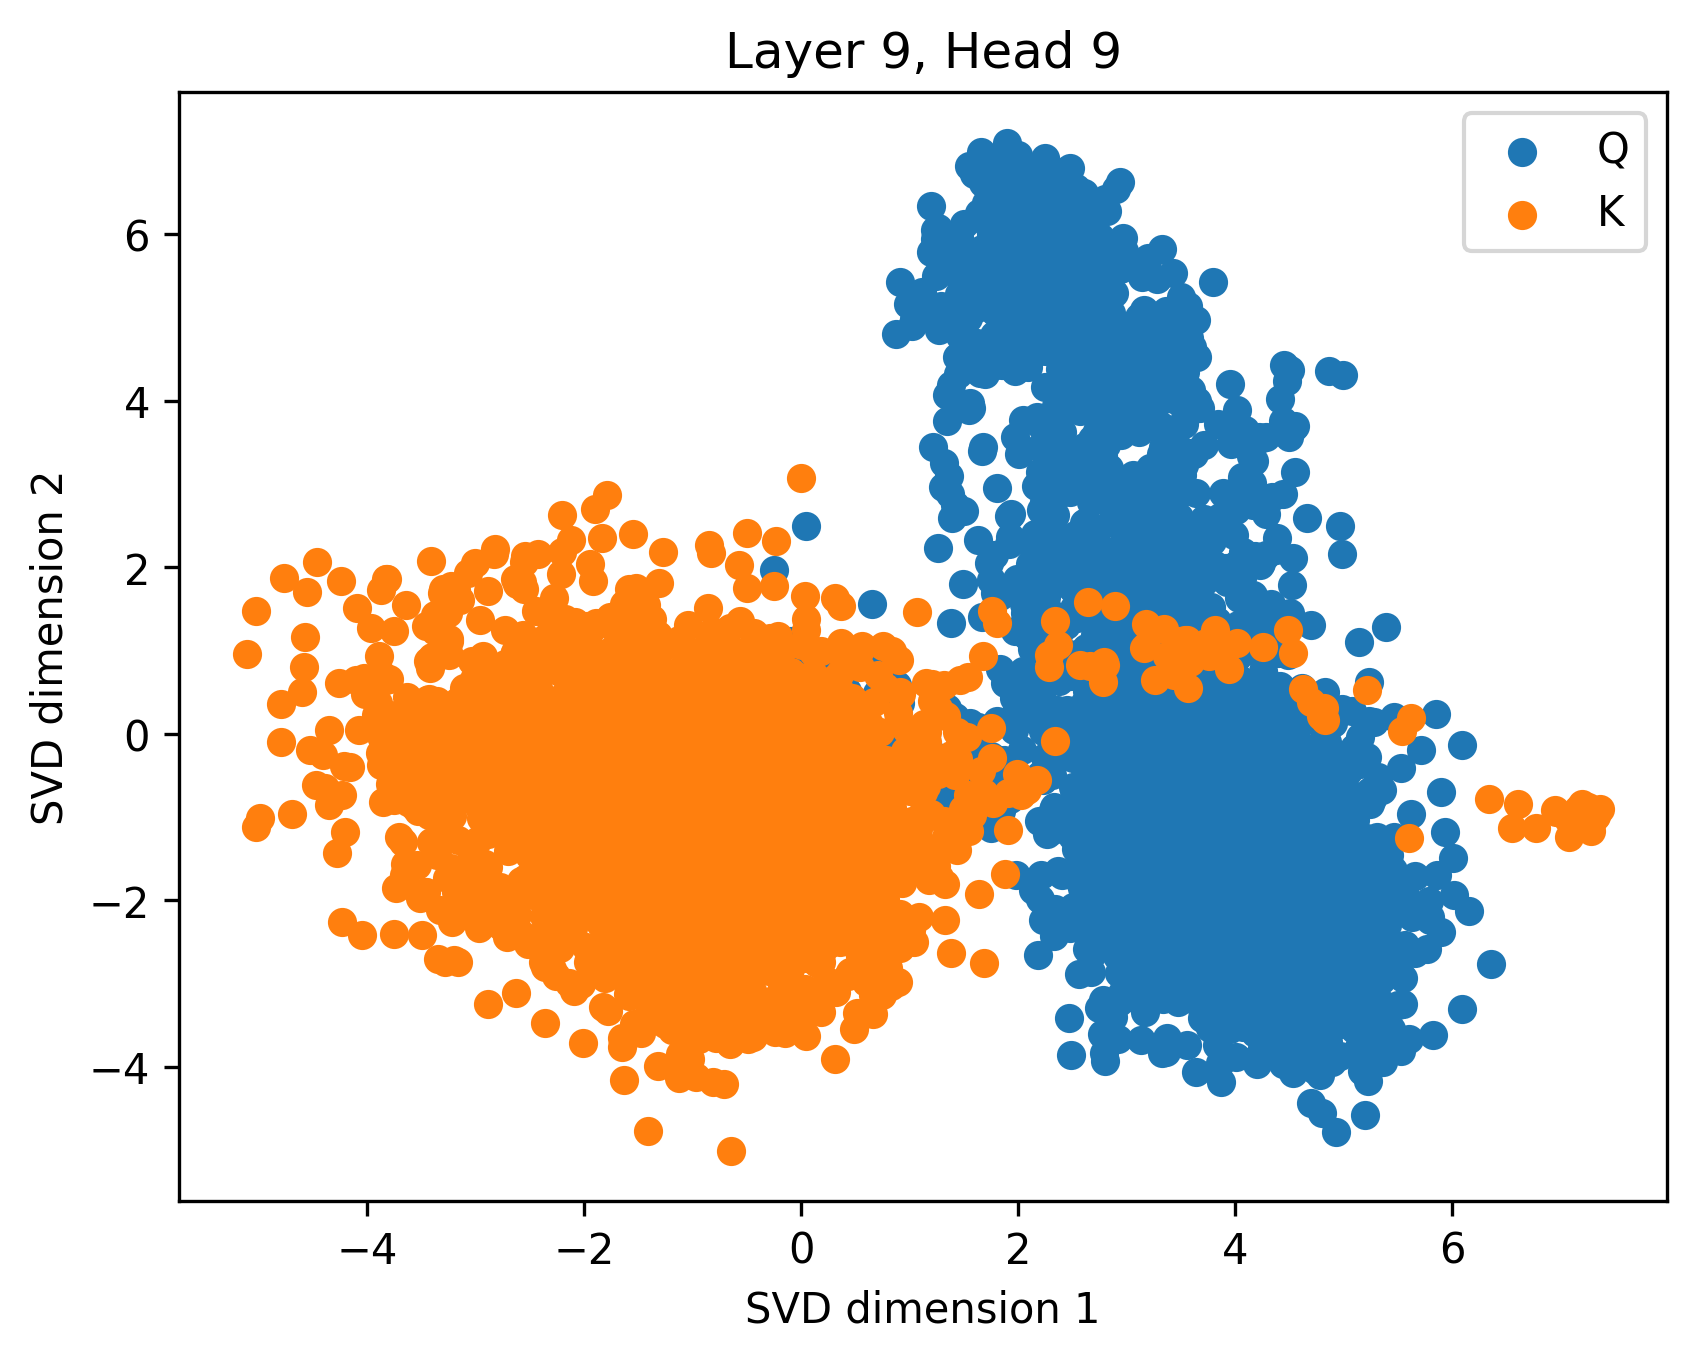
\includegraphics[width=\linewidth]{sources/part_1/anisotropy/imgs/dist_l9h9_s200_Q.png}
         \caption{Step 200k}
         \label{fig:dist_qk_s200_Q}
    \end{subfigure}
    \begin{subfigure}[b]{0.24\linewidth}
         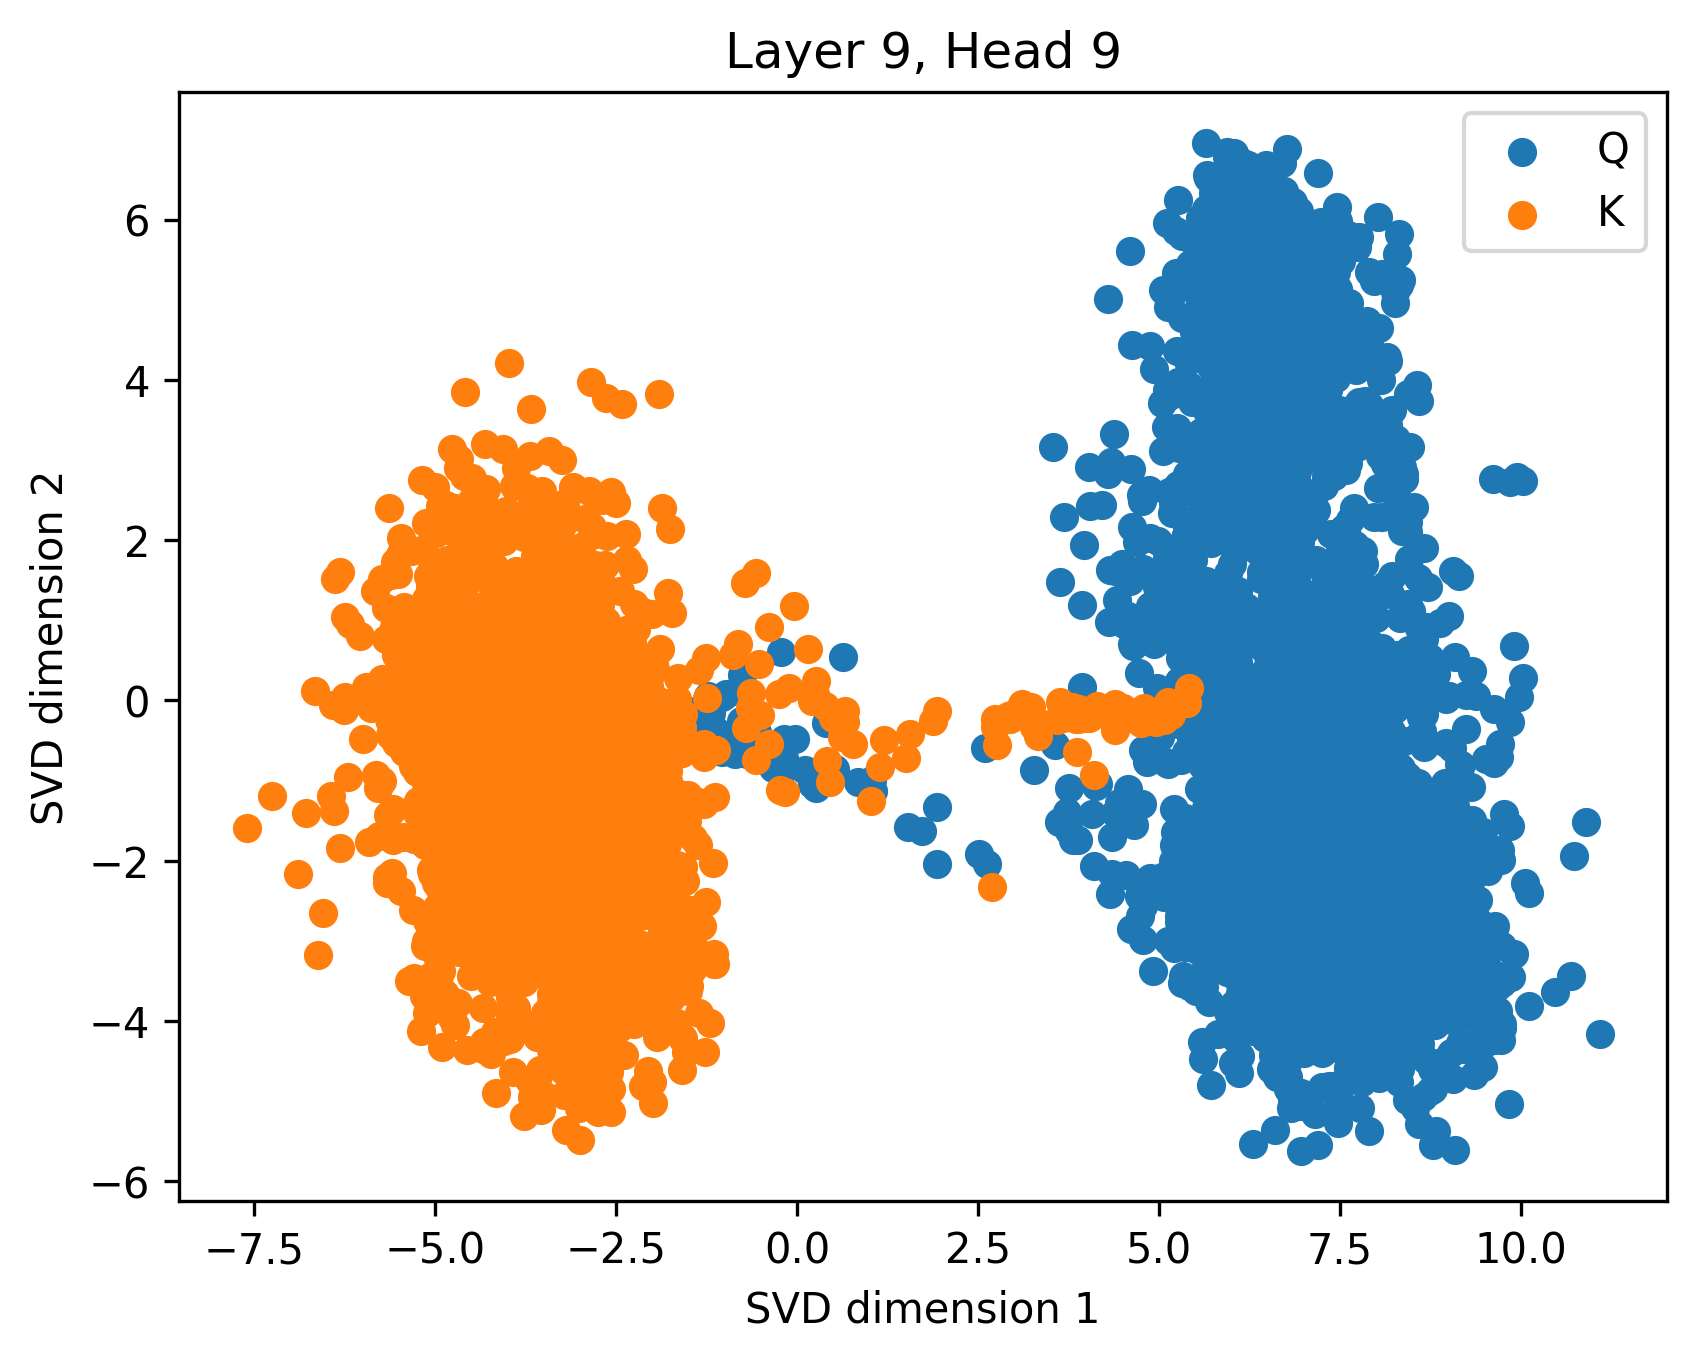
\includegraphics[width=\linewidth]{sources/part_1/anisotropy/imgs/dist_l9h9_s2000_Q.png}
         \caption{Step 2M (final)}
         \label{fig:dist_qk_s2M_Q}
    \end{subfigure}
    \caption{Evolution of $Q^h_s$ and $K^h_s$ distributions along training. Vectors are projected using the SVD computed on $Q^h_s$.}
    \label{fig:proj_qk_heads_Q}
\end{figure*}

\begin{figure}[ht!]
    \centering
    \begin{subfigure}[b]{0.48\columnwidth}
         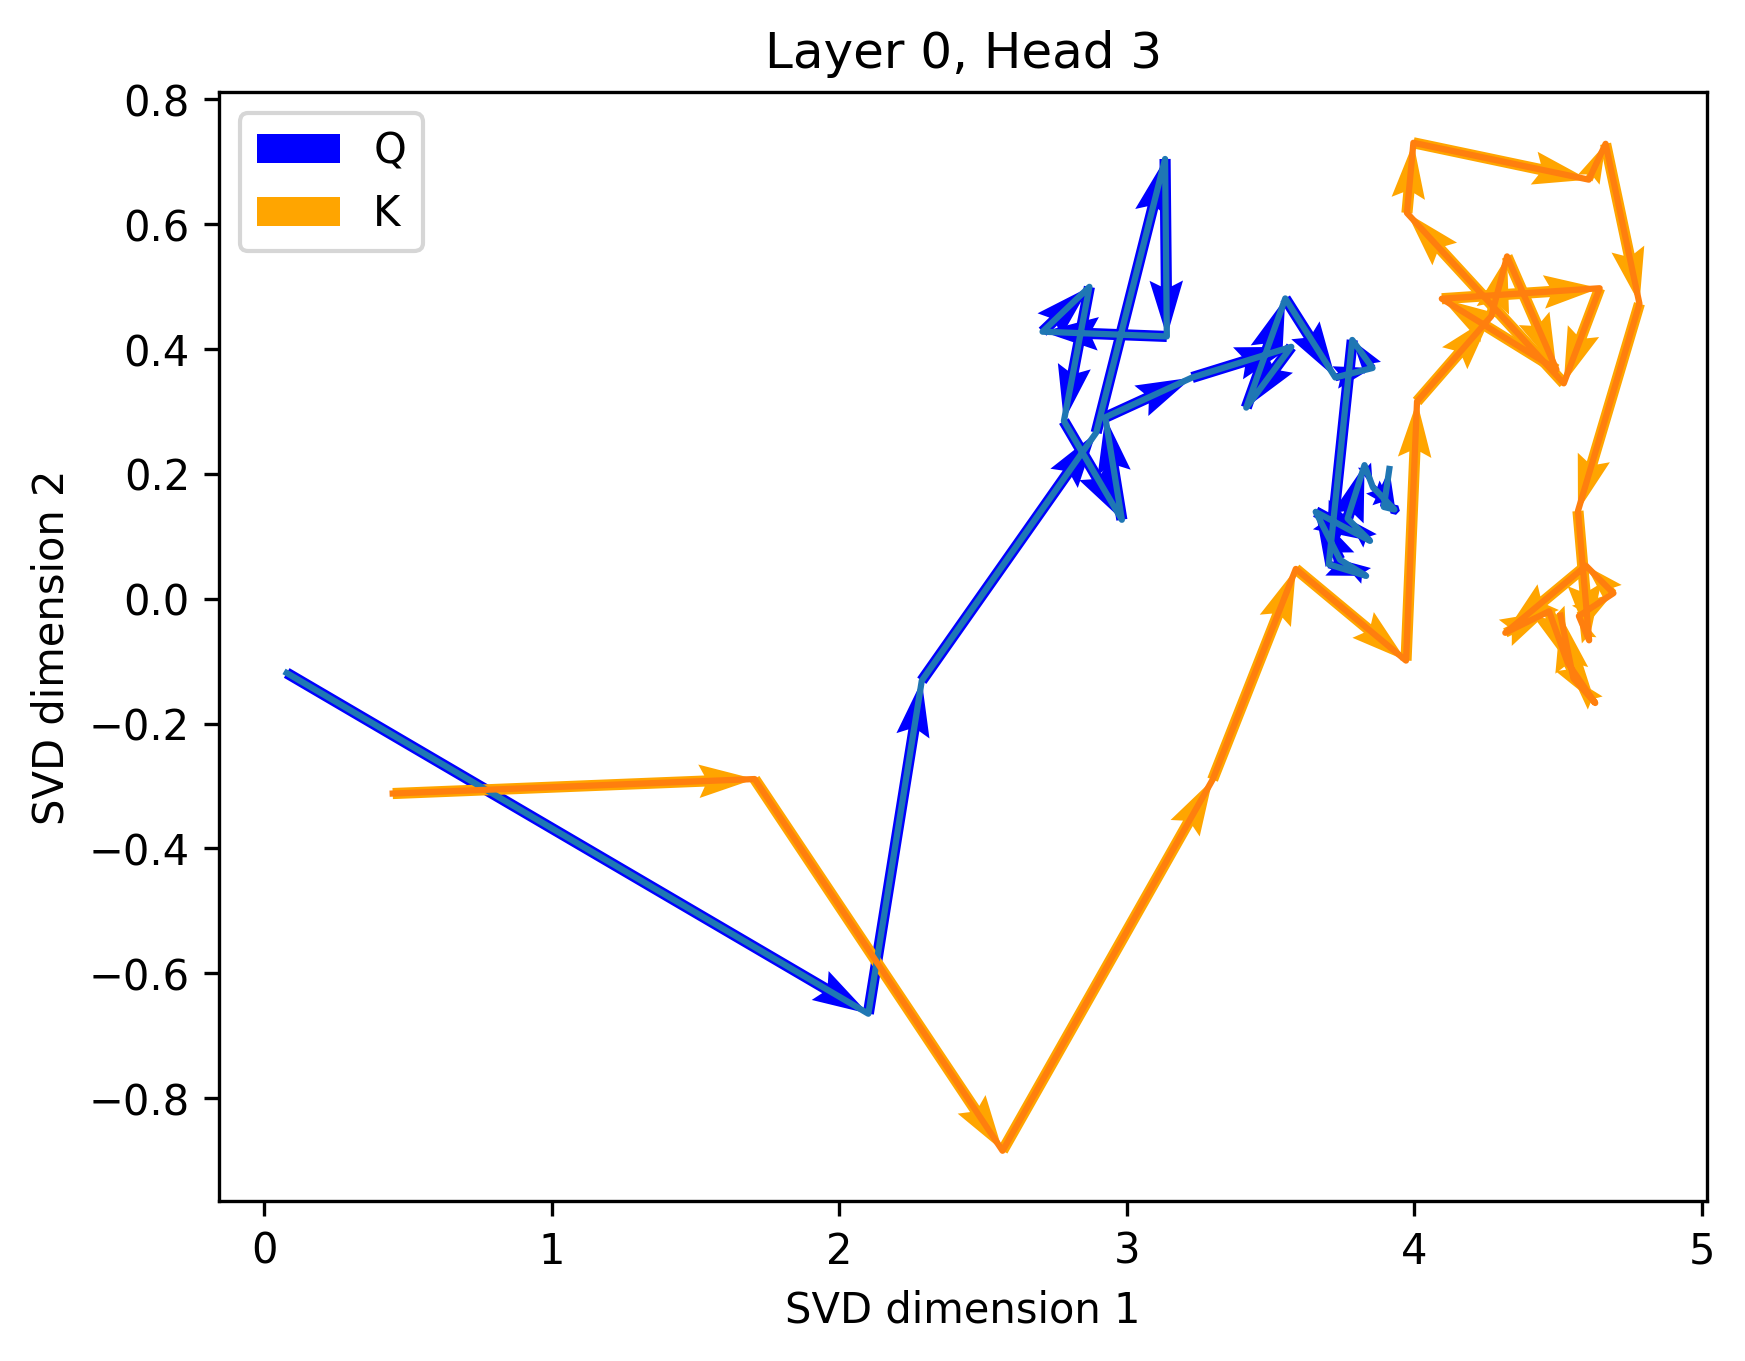
\includegraphics[width=\linewidth]{sources/part_1/anisotropy/imgs/l0h3_samedir_QK_K.png}
         \caption{Similar}
         \label{fig:QK_simdir_K}
    \end{subfigure}
    \begin{subfigure}[b]{0.48\columnwidth}
         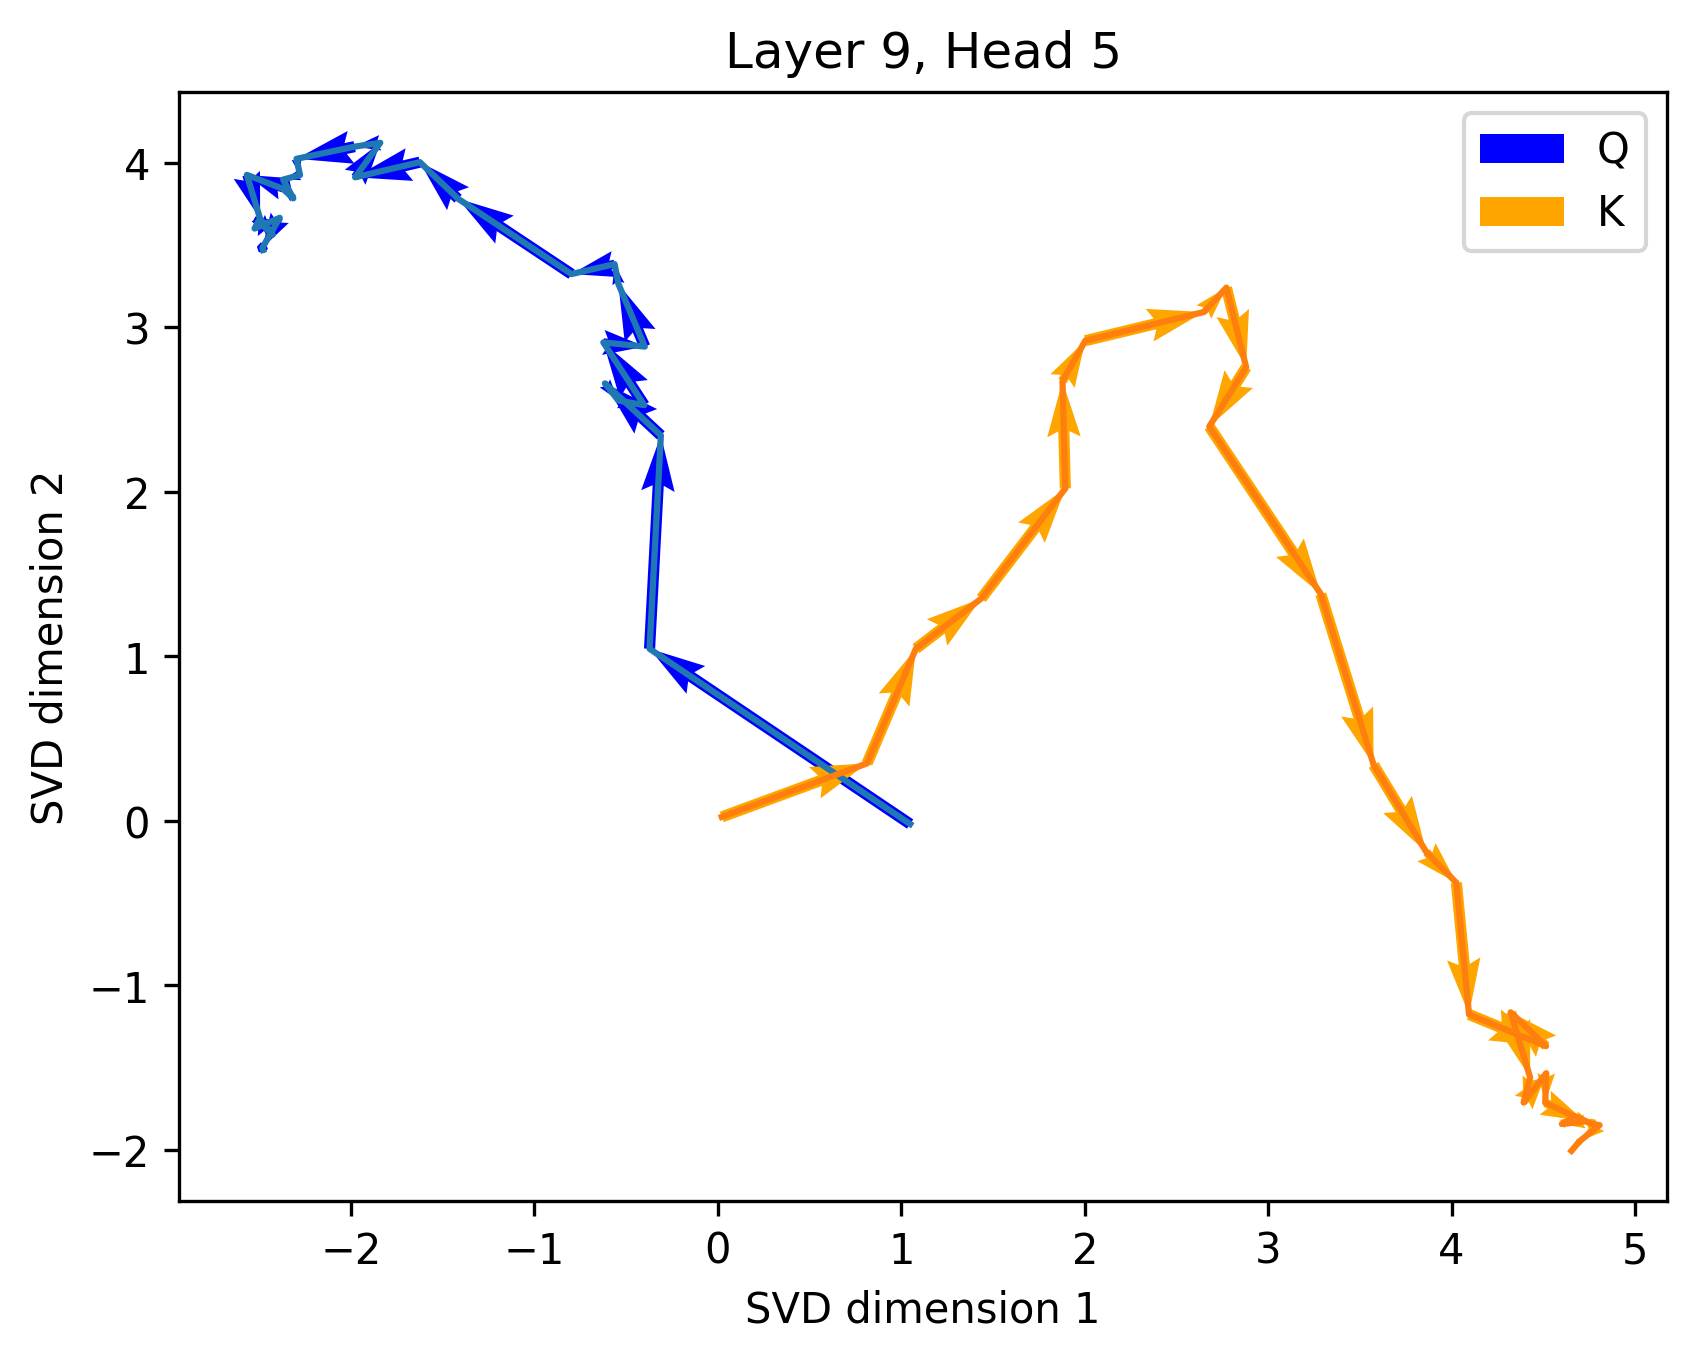
\includegraphics[width=\linewidth]{sources/part_1/anisotropy/imgs/l9h5_diffdir_QK_K.png}
         \caption{Opposite}
         \label{fig:QK_diffdir_K}
    \end{subfigure}
    \caption{Evolution of $\bar{Q^h_s}$ and $\bar{K^h_s}$ along training for two different heads in the network, projected via the SVD of $K^h_s$.
    }
    \label{fig:QK_dir_K}
\end{figure}

\begin{figure}[ht!]
    \centering
    \begin{subfigure}[b]{0.48\columnwidth}
         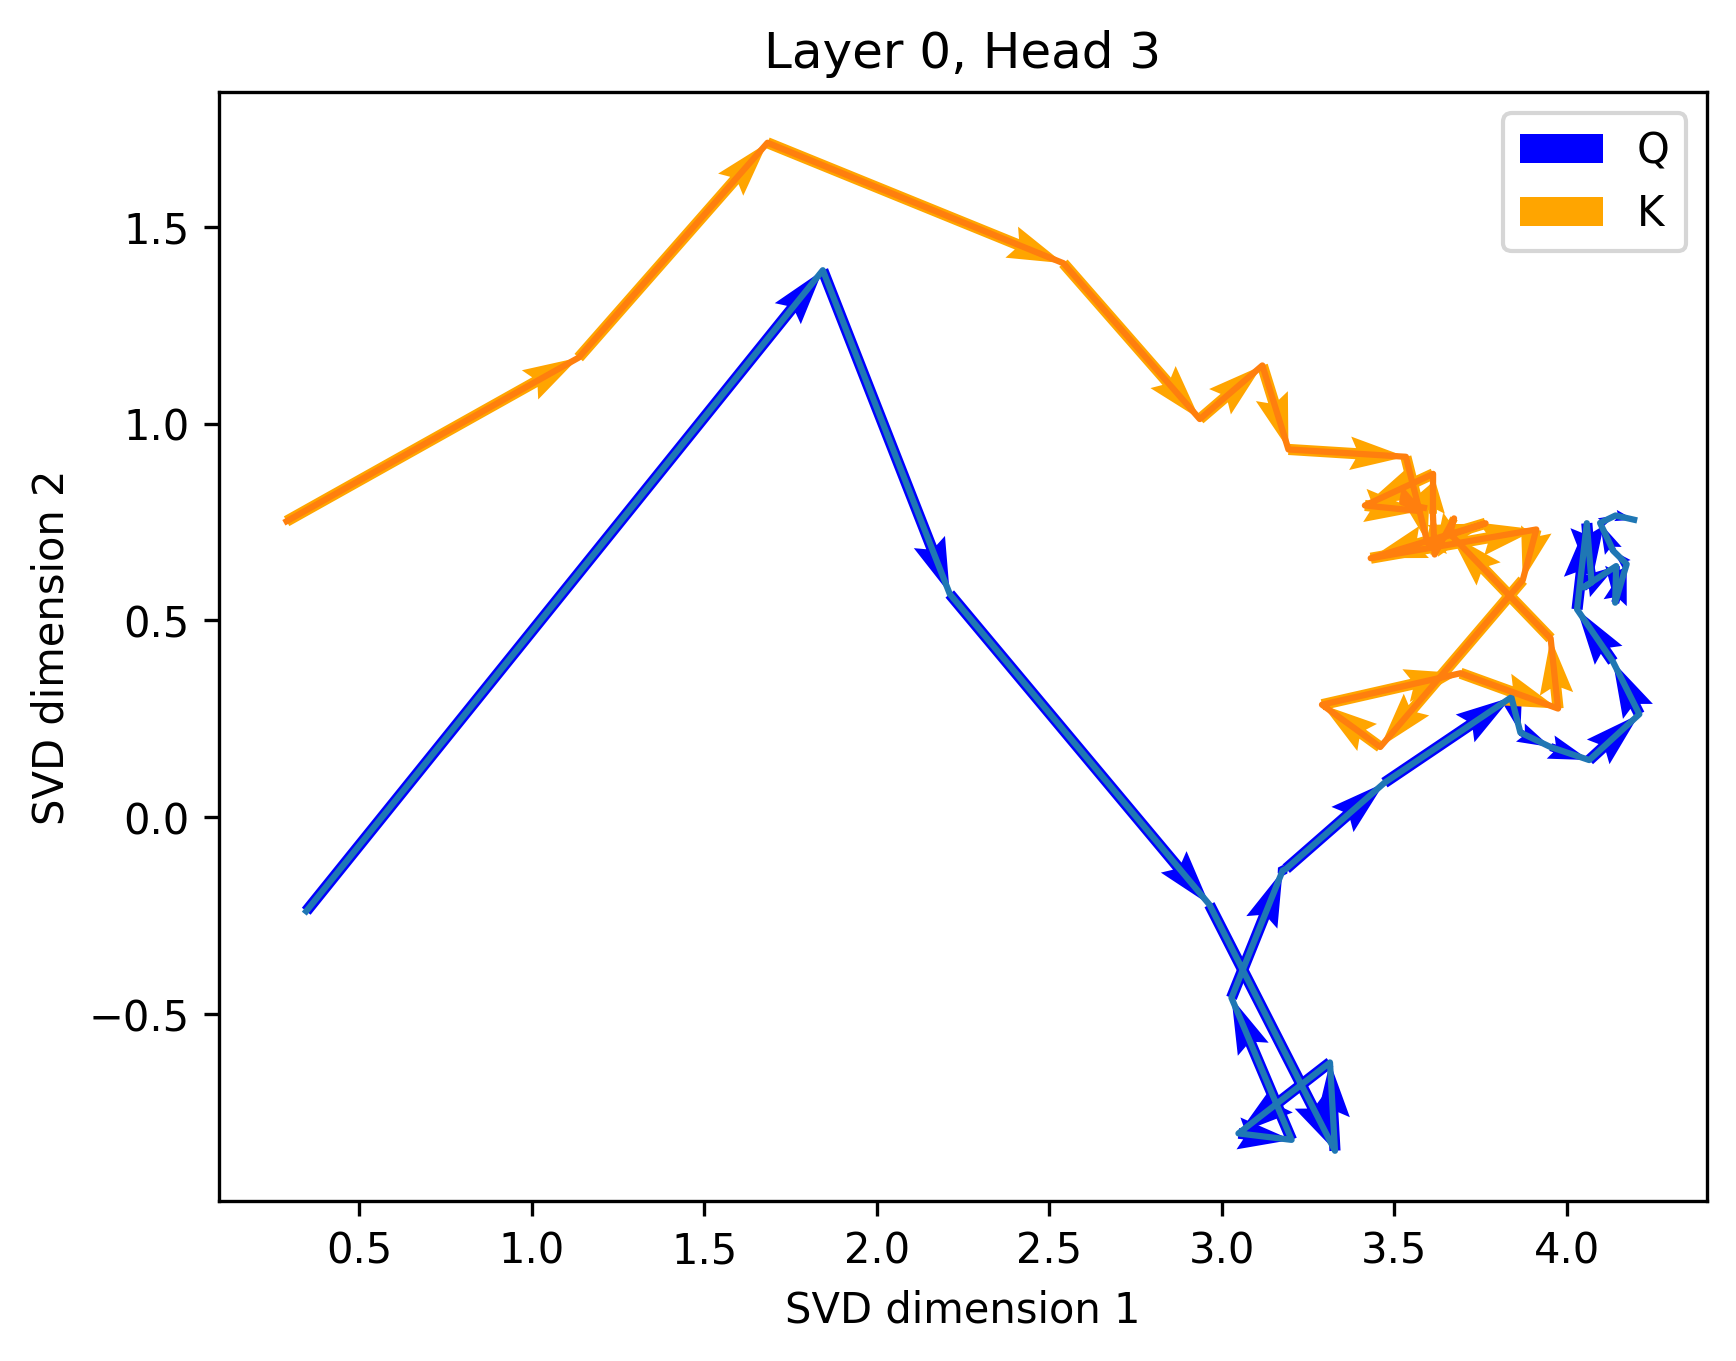
\includegraphics[width=\linewidth]{sources/part_1/anisotropy/imgs/l0h3_samedir_QK_Q.png}
         \caption{Similar}
         \label{fig:QK_simdir_Q}
    \end{subfigure}
    \begin{subfigure}[b]{0.48\columnwidth}
         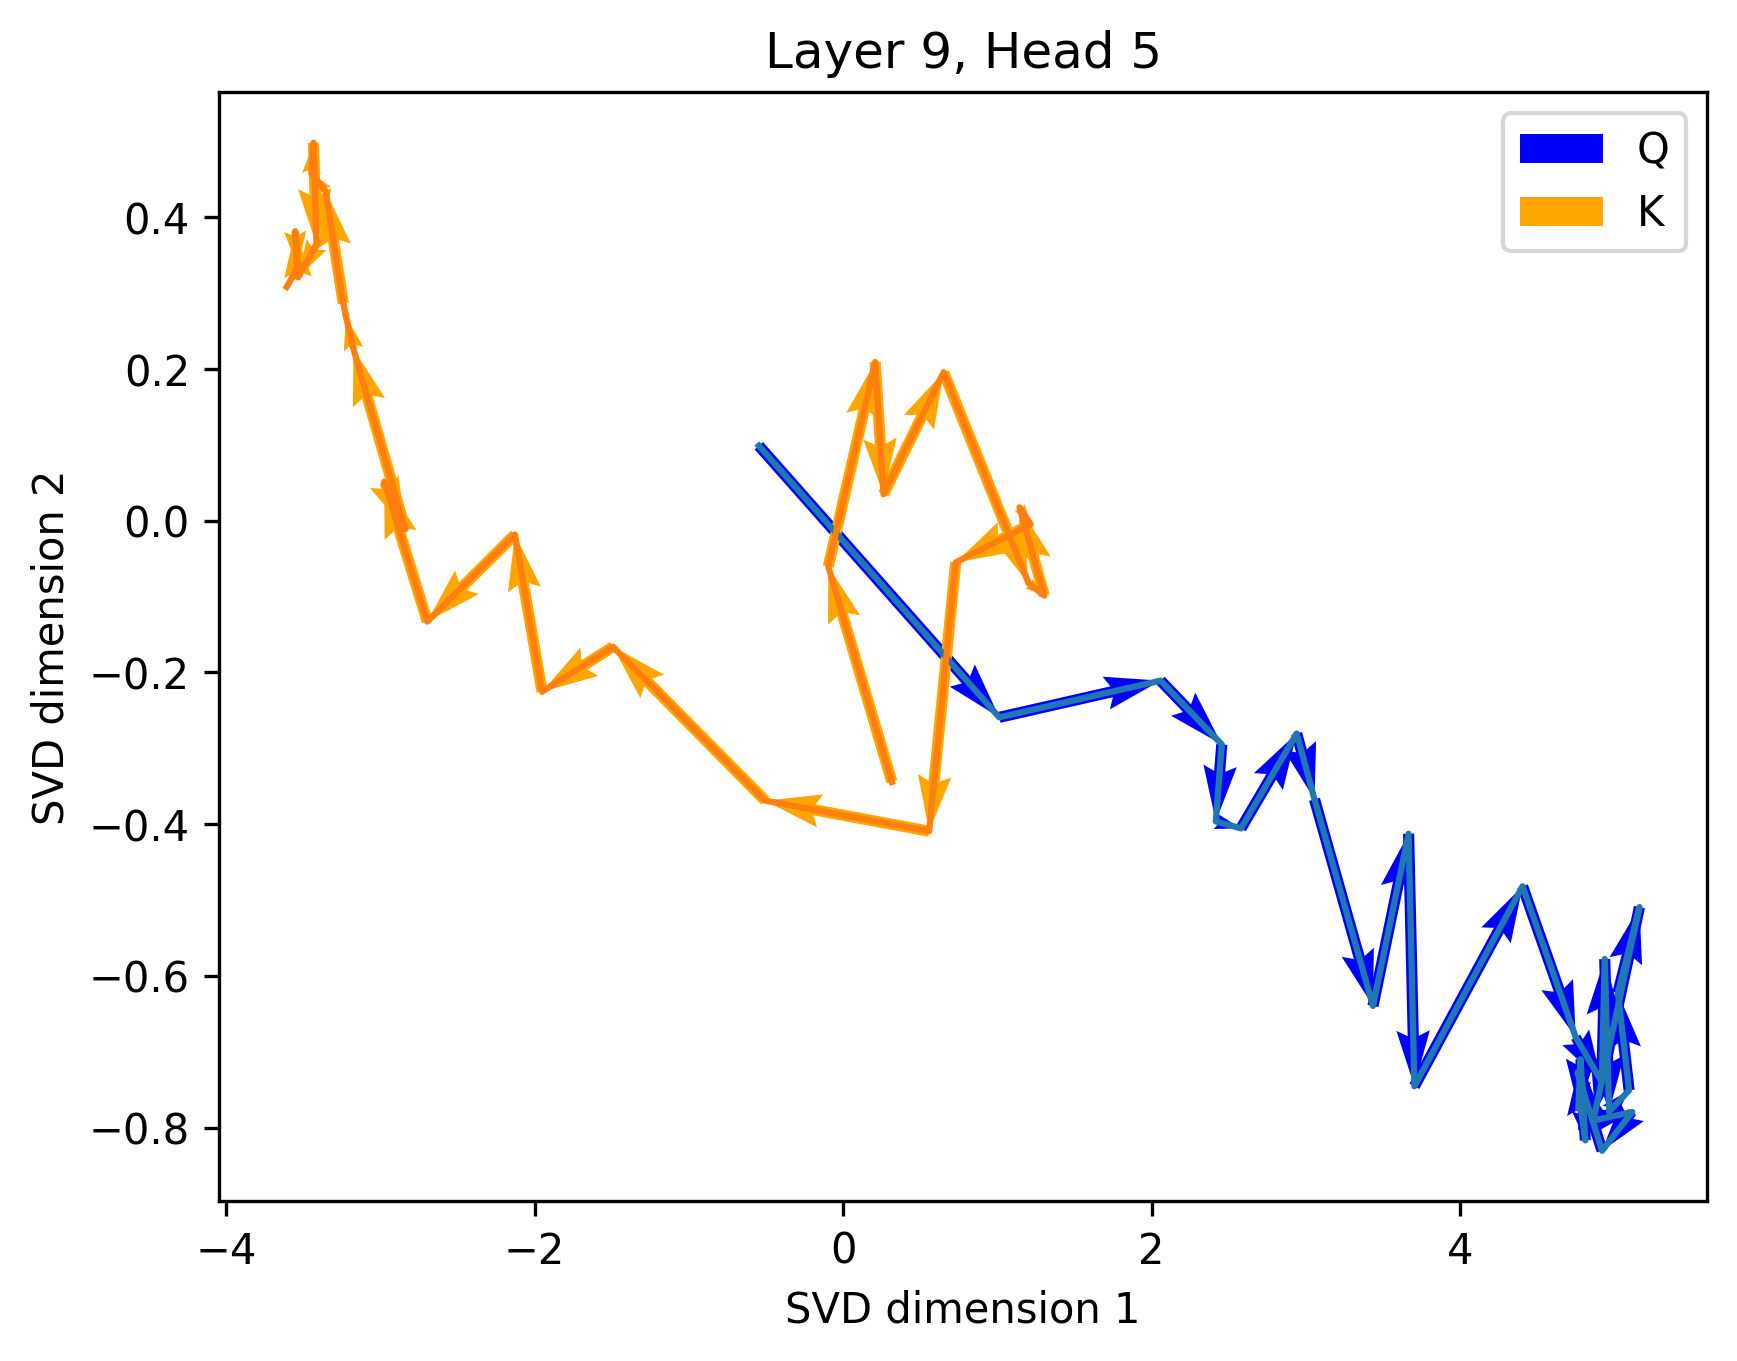
\includegraphics[width=\linewidth]{sources/part_1/anisotropy/imgs/l9h5_diffdir_QK_Q.png}
         \caption{Opposite}
         \label{fig:QK_diffdir_Q}
    \end{subfigure}
    \caption{Evolution of $\bar{Q^h_s}$ and $\bar{K^h_s}$ along training for two different heads in the network, projected via the SVD of $Q^h_s$.}
    \label{fig:QK_dir_Q}
\end{figure}

\subsection{Stability across MultiBERT seeds}
\begin{figure*}[ht]
    \centering
    \begin{subfigure}[b]{0.24\linewidth}
         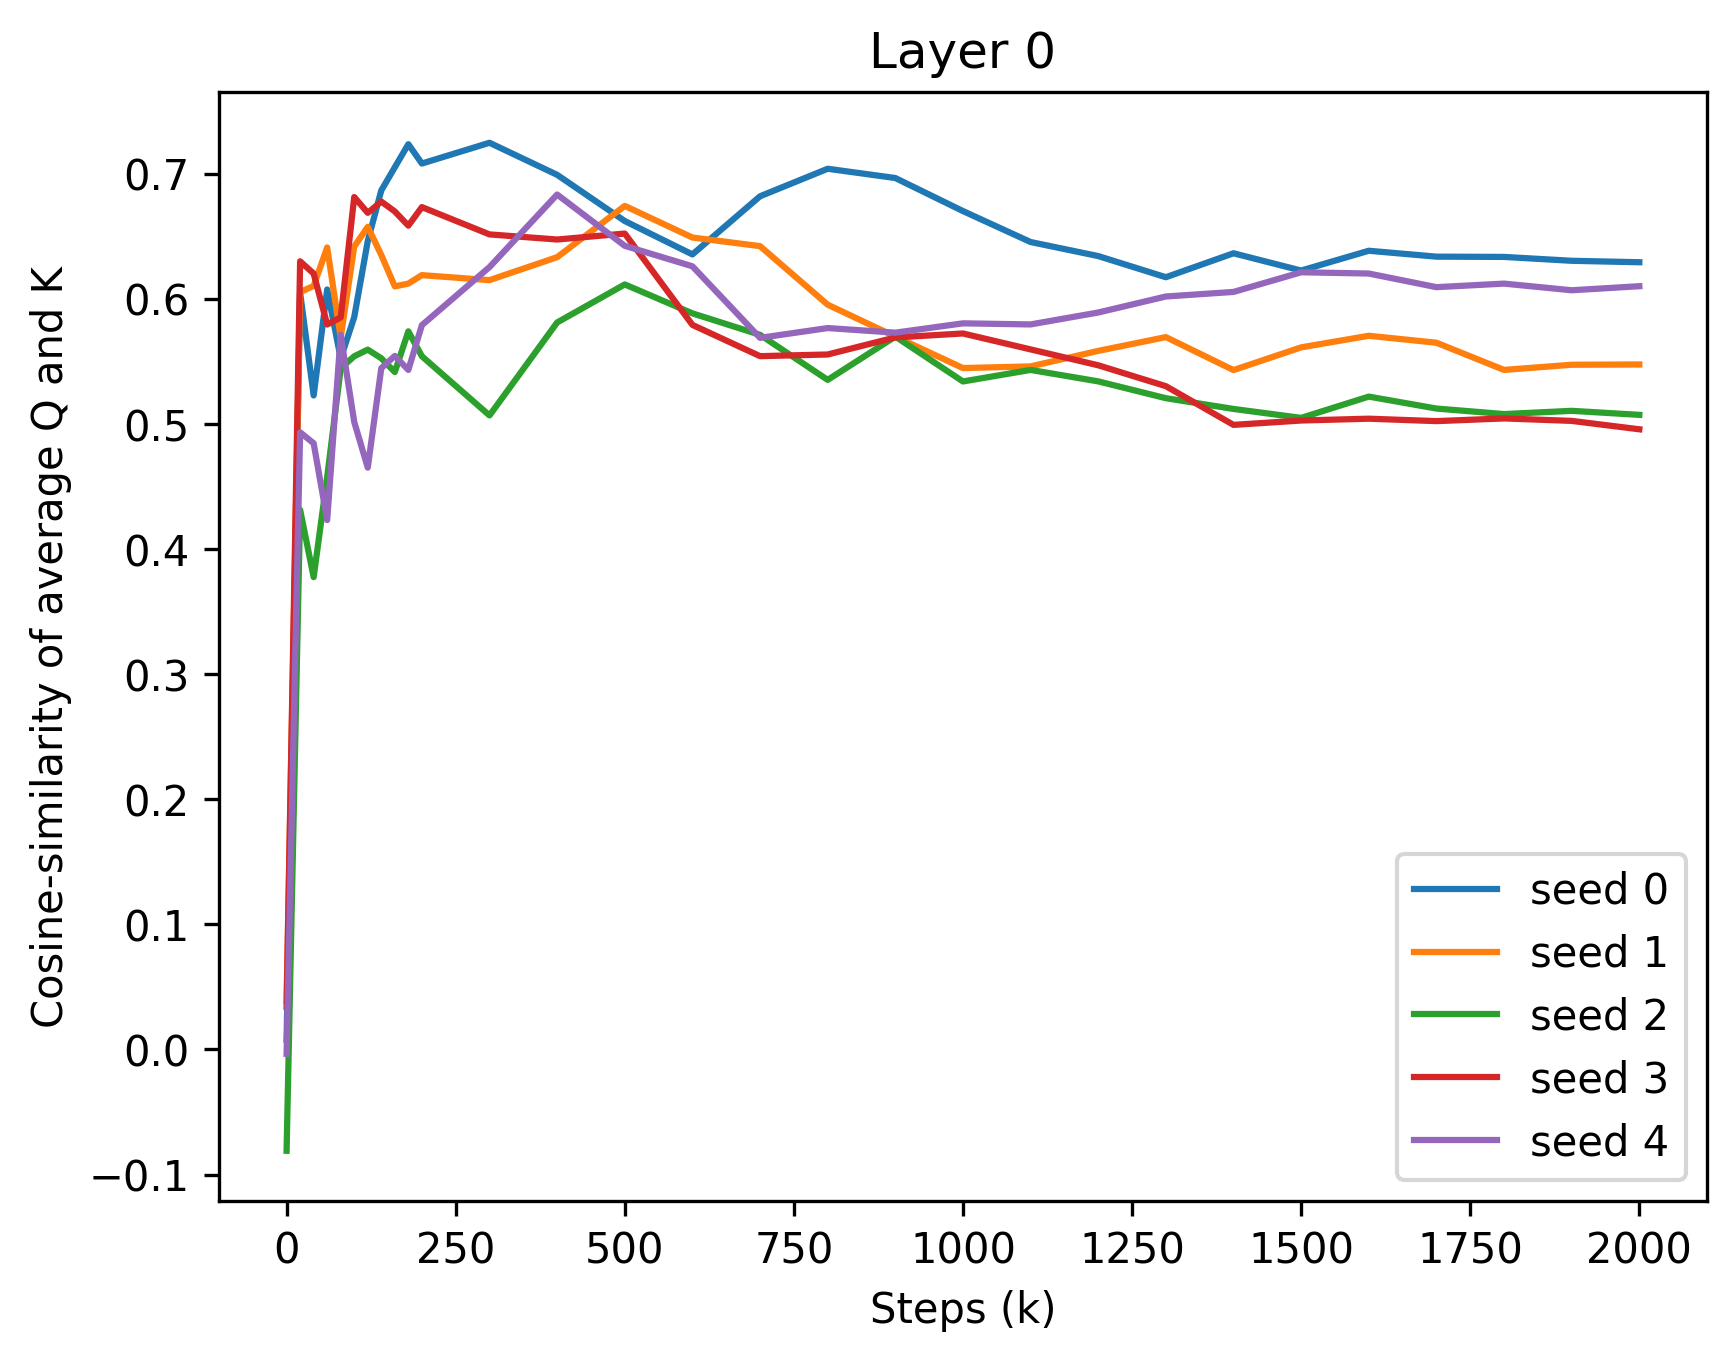
\includegraphics[width=\linewidth]{sources/part_1/anisotropy/imgs/seeds_qk_l0.png}
         \caption{Layer 0}
         \label{fig:seeds_l0}
    \end{subfigure}
    \begin{subfigure}[b]{0.24\linewidth}
         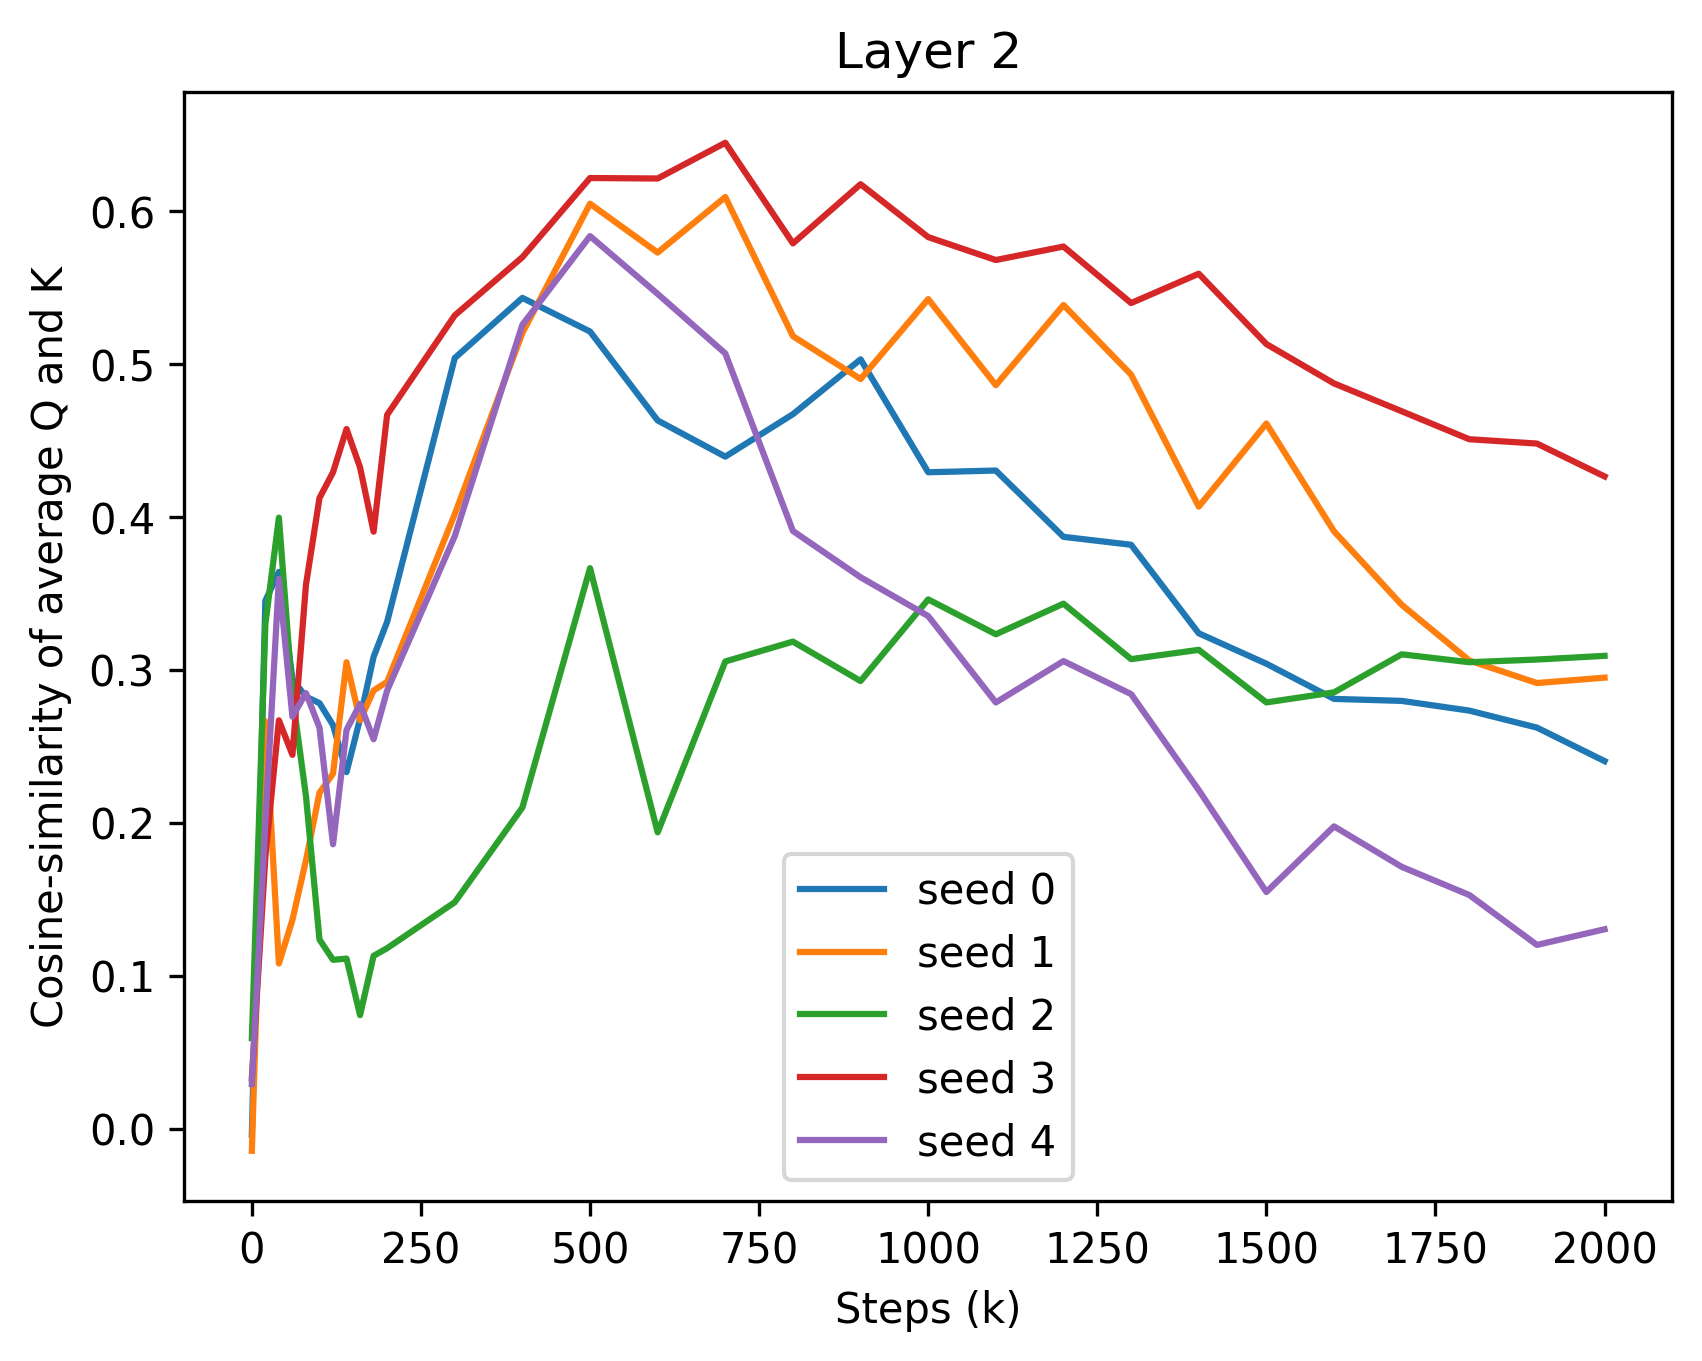
\includegraphics[width=\linewidth]{sources/part_1/anisotropy/imgs/seeds_qk_l2.png}
         \caption{Layer 2}
         \label{fig:seeds_l2}
    \end{subfigure}
    \begin{subfigure}[b]{0.24\linewidth}
         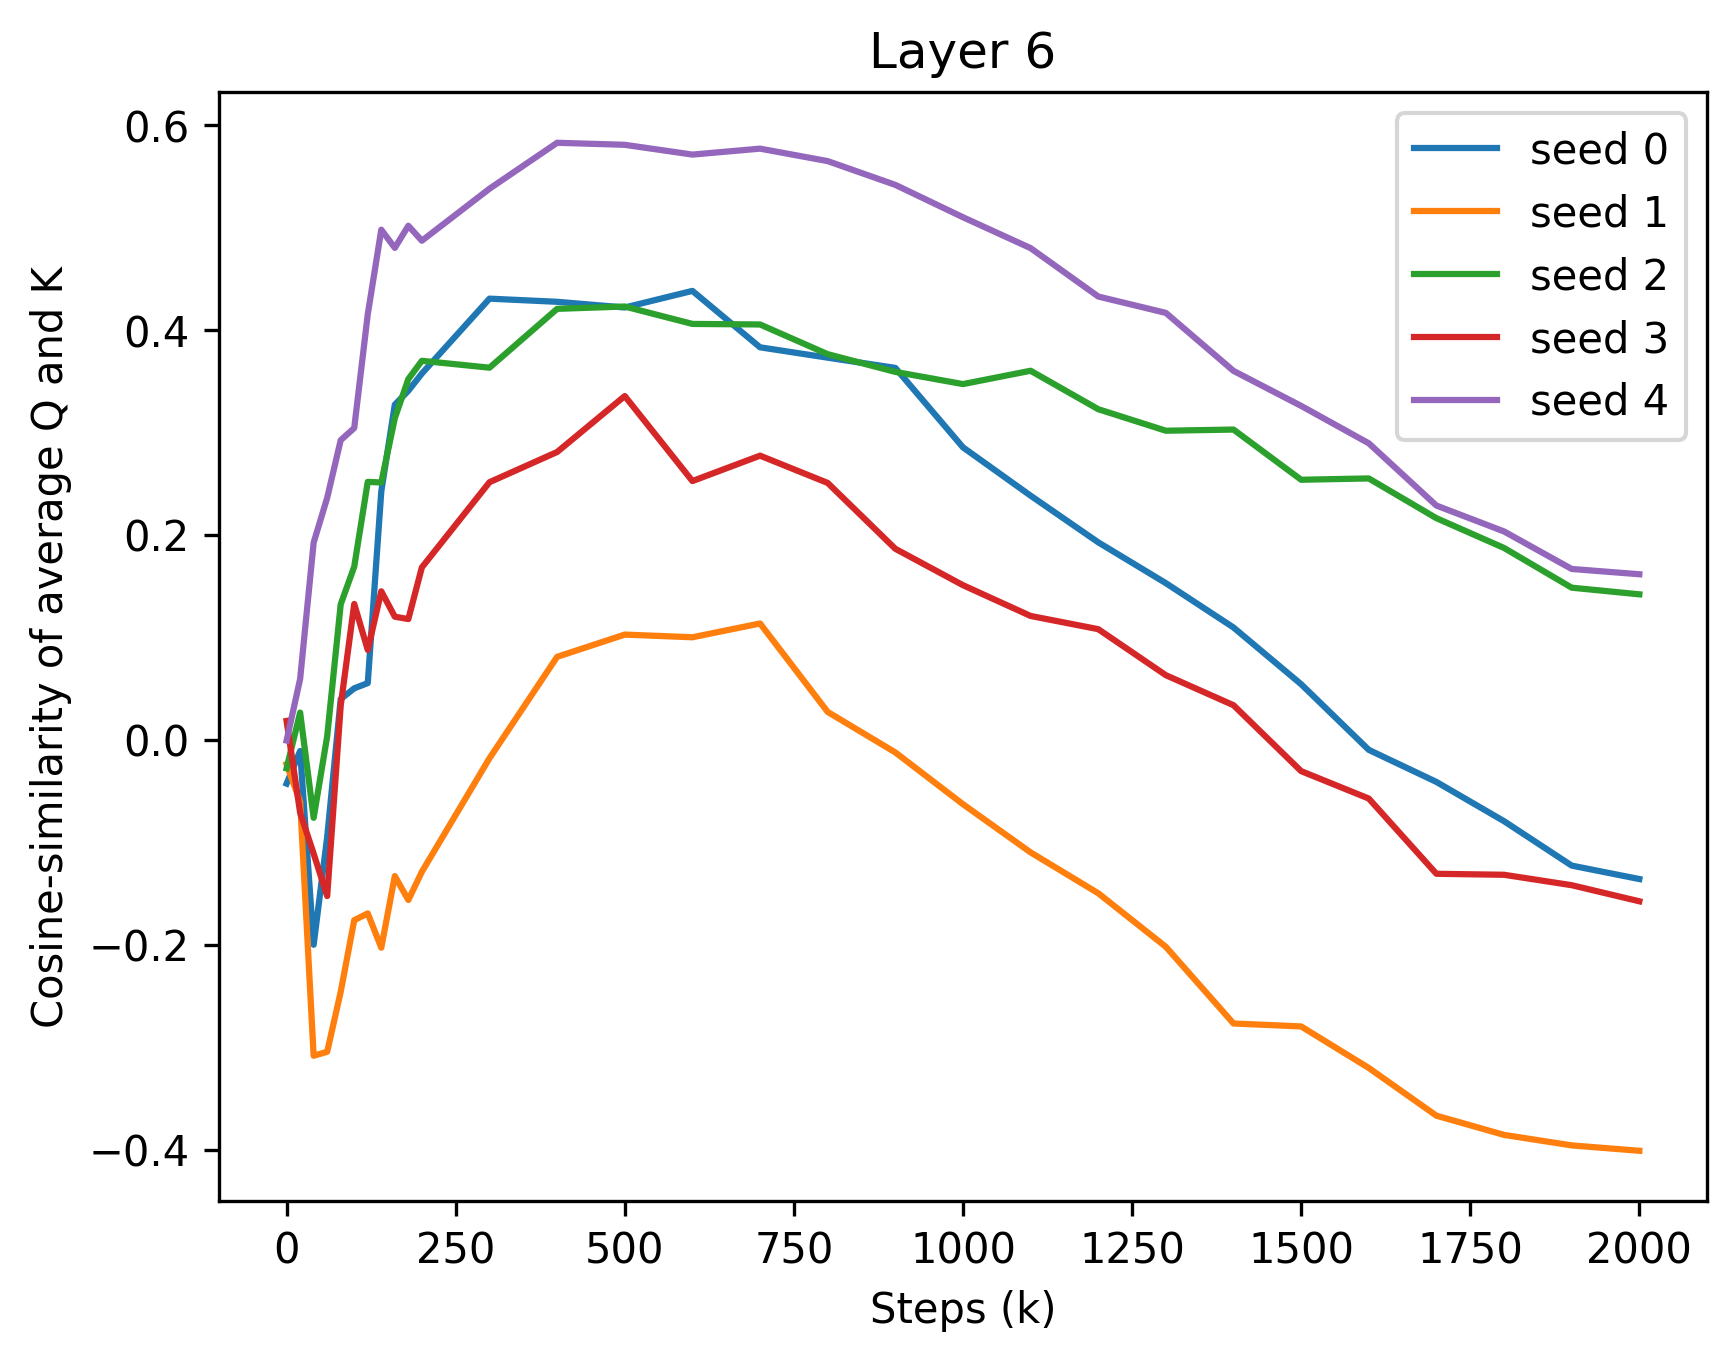
\includegraphics[width=\linewidth]{sources/part_1/anisotropy/imgs/seeds_qk_l6.png}
         \caption{Layer 6}
         \label{fig:seeds_l6}
    \end{subfigure}
    \begin{subfigure}[b]{0.24\linewidth}
         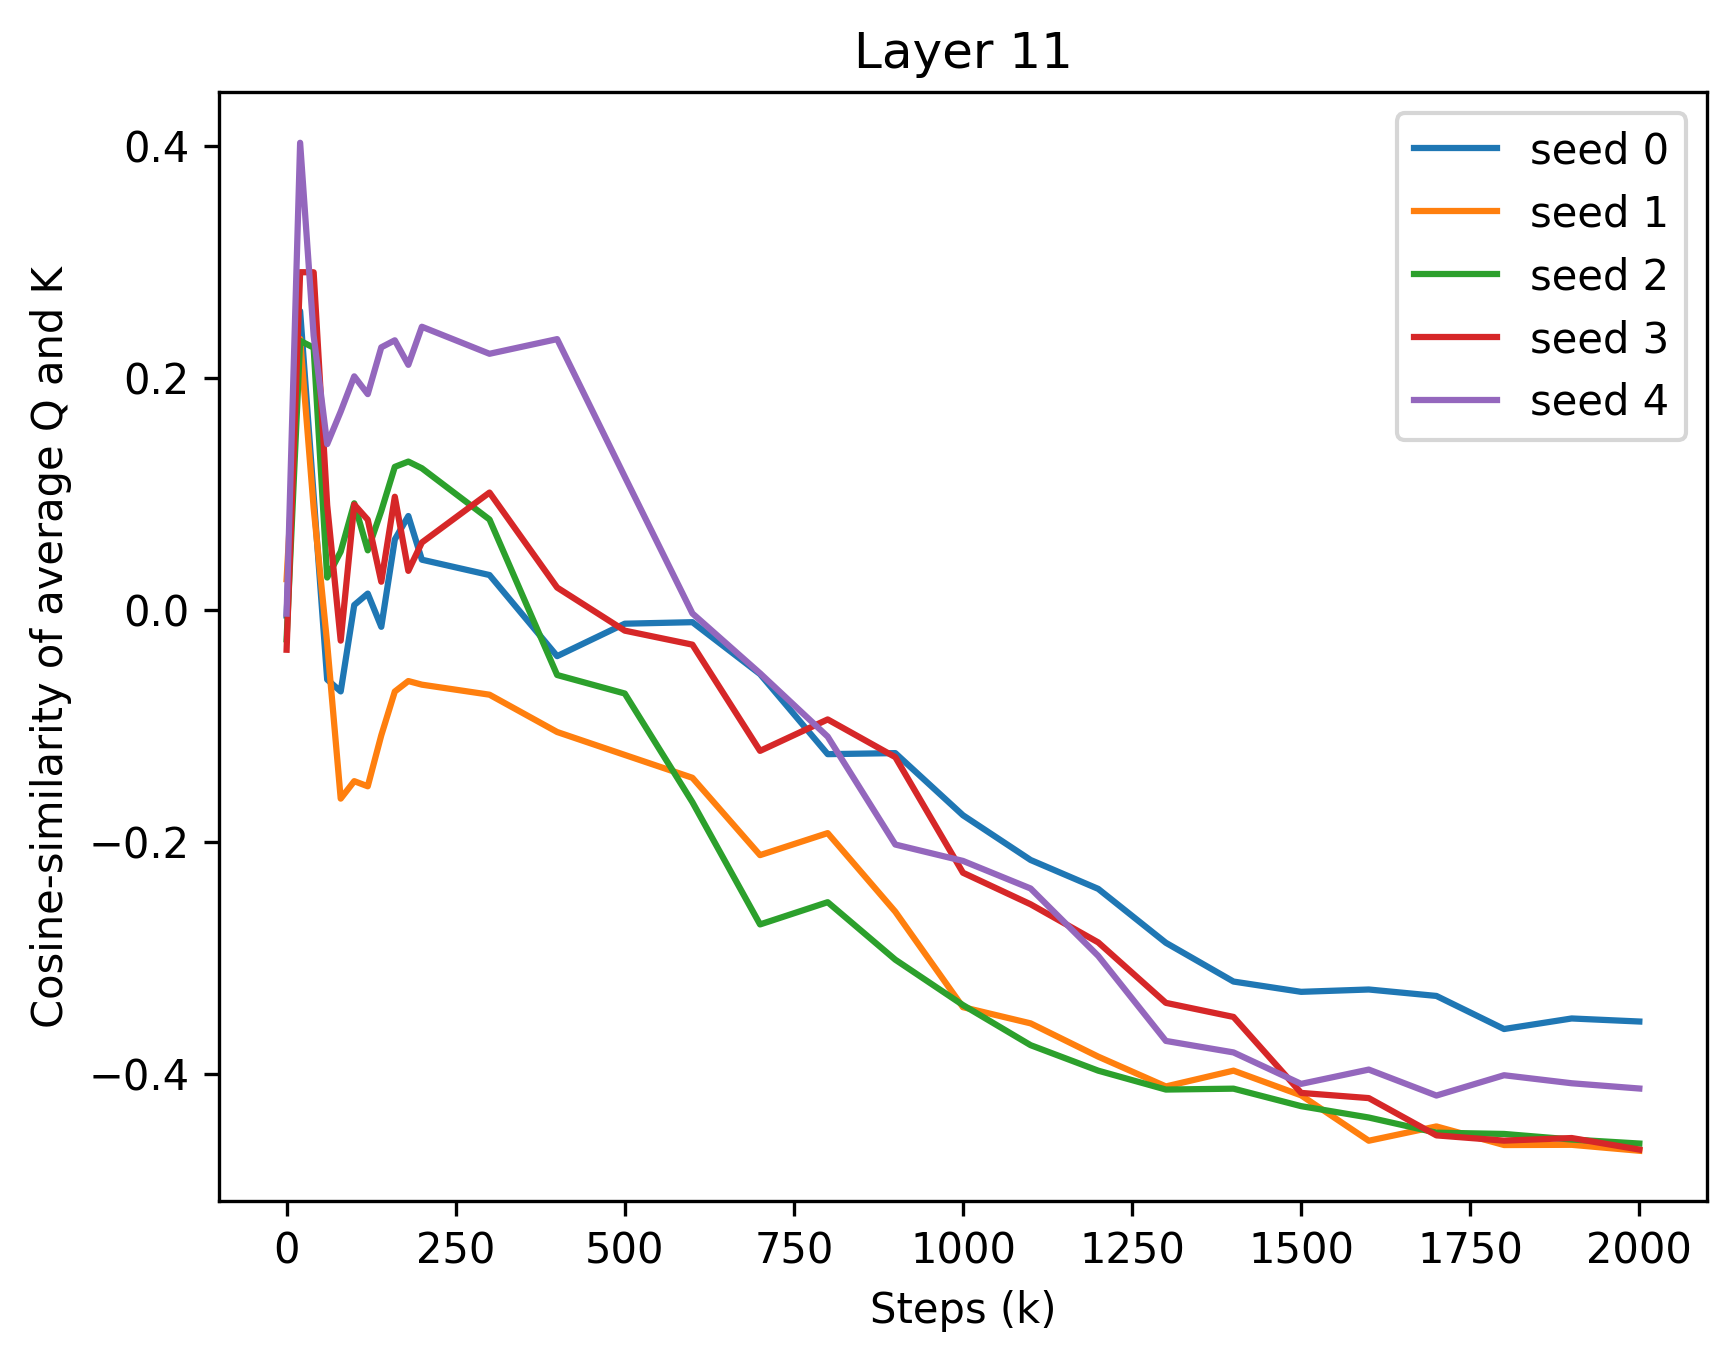
\includegraphics[width=\linewidth]{sources/part_1/anisotropy/imgs/seeds_qk_l11.png}
         \caption{Layer 11}
         \label{fig:seeds_l11}
    \end{subfigure}
    \caption{Evolution of cosine-similarity between $\bar{Q^h_s}$ and $\bar{K^h_s}$ along training for various initialization seeds. Representations are concatenated across heads, and each color represents one seed of the MultiBERT models. We observe similar trends across seeds.}
    \label{fig:seeds_qk}
\end{figure*}

\clearpage

\section{Pretraining hyperparameters for \Cref{chap:headless_lm}}
\label{app:train_hp}

\subsection{Monolingual encoders}
\label{app:train_mono_enc}
\begin{table}[H]
\centering
\small
\begin{tabular}{c|c}
\toprule
Dataset & OpenWebText2  \\ \hline
Architecture & \texttt{bert-base-uncased} \\ \hline
Tokenizer & \texttt{pythia-70m-deduped} \\ \hline
Optimizer         & AdamW      \\ \hline
Learning rate     & 1e-4       \\ \hline
Precision  & 16 \\ \hline
Weight decay      & 0.01       \\ \hline
Gradient clipping & 1          \\ \hline
Device batch size        & 32 / 64         \\ \hline
Batch size        & 256 / 512         \\ \hline
Sequence length   & 128        \\ \hline
LR schedule       & Triangular \\ \hline
Warmup steps      & 10000      \\ \hline
Nb. steps         & 1000000        \\ \bottomrule
\end{tabular}
\caption{Pre-training hyperparameters used for the monolingual encoders. When they differ between vanilla and headless models, we provide separate values formatted as (vanilla / headless). Model names written as \texttt{model-name} refer to their HuggingFace release.}
\end{table}

\subsection{Monolingual decoders}
\label{app:train_mono_dec}
\begin{table}[H]
\centering
\small
\begin{tabular}{c|c}
\toprule
Dataset & OpenWebText2  \\ \hline
Architecture & \texttt{pythia-70m-deduped} \\ \hline
Tokenizer & \texttt{pythia-70m-deduped} \\ \hline
Optimizer         & AdamW      \\ \hline
Adam $\epsilon$ & 1e-8   \\ \hline
Adam $(\beta_1, \beta_2)$ & (0.9, 0.95)   \\ \hline
Learning rate     & 1e-3       \\ \hline
Precision  & 16 \\ \hline
Weight decay      & 0.1       \\ \hline
Gradient clipping & 1          \\ \hline
Device batch size        & 8 / 8         \\ \hline
Batch size        & 1024 / 1024         \\ \hline
Sequence length   & 2048        \\ \hline
LR schedule       & Cosine \\ \hline
Warmup steps      & 1430      \\ \hline
Nb. steps         & 143000        \\ \bottomrule
\end{tabular}
\caption{Pre-training hyperparameters used for the monolingual encoders. When they differ between vanilla and headless models, we provide separate values formatted as (vanilla / headless).}
\end{table}

\subsection{Multilingual encoders}
\label{app:train_multi_enc}


\begin{table}[H]
\centering
\small
\begin{tabular}{c|c}
\toprule
Dataset & Wikipedia (multilingual)  \\ \hline
Architecture & \texttt{distilbert-base-multilingual-cased} \\ \hline
Tokenizer & \texttt{distilbert-base-multilingual-cased} \\ \hline
Optimizer         & AdamW      \\ \hline
Learning rate     & 2e-4       \\ \hline
Precision  & 16 \\ \hline
Weight decay      & 0.01       \\ \hline
Gradient clipping & 1          \\ \hline
Device batch size        & 64         \\ \hline
Batch size        & 64        \\ \hline
Sequence length   & 128        \\ \hline
LR schedule       & Triangular \\ \hline
Warmup steps      & 10000      \\ \hline
Nb. steps         & 400000        \\ \bottomrule
\end{tabular}
\caption{Pre-training hyperparameters used for the multilingual encoders.}
\end{table}

\subsection{Small monolingual encoders}
\label{app:s_train_mono_enc}


\begin{table}[H]
\centering
\small
\begin{tabular}{c|c}
\toprule
Dataset & CC-News  \\ \hline
Architecture & \texttt{google/bert\_uncased\_L-4\_H-512\_A-8} \\ \hline
Tokenizer & \texttt{google/bert\_uncased\_L-4\_H-512\_A-8} \\ \hline
Optimizer         & AdamW      \\ \hline
Learning rate     & 2e-4       \\ \hline
Precision  & 16 \\ \hline
Weight decay      & 0.01       \\ \hline
Gradient clipping & 1          \\ \hline
Device batch size        & 64         \\ \hline
Batch size        & 64        \\ \hline
Sequence length   & 128        \\ \hline
LR schedule       & Triangular \\ \hline
Warmup steps      & 10000      \\ \hline
Nb. steps         & 400000        \\ \bottomrule
\end{tabular}
\caption{Pre-training hyperparameters used for the small monolingual encoders used in \Cref{fig:tokencount}.}
\end{table}

\subsection{Small monolingual decoders}
\label{app:s_train_mono_dec}


\begin{table}[H]
\centering
\small
\begin{tabular}{c|c}
\toprule
Dataset & CC-News \\ \hline
Architecture & \texttt{gpt2} \\ \hline
Hidden size & 192 \\ \hline
Number heads & 3 \\ \hline
Number layers & 3 \\ \hline
Tokenizer & \texttt{gpt2} \\ \hline
Optimizer         & AdamW      \\ \hline
Learning rate     & 2.5e-4       \\ \hline
Precision  & 16 \\ \hline
Weight decay      & 0.01       \\ \hline
Gradient clipping & 1          \\ \hline
Sequence length   & 128        \\ \hline
LR schedule       & Cosine \\ \hline
Warmup steps      & 2000      \\ \hline
Nb. steps         & 1000000        \\ \bottomrule
\end{tabular}
\caption{Pre-training hyperparameters used for the small monolingual decoders used in \Cref{fig:batch_size}. These models rely on the GPT-2 architecture with a few changes. These changes scale down the model size to 11M parameters.}
\end{table}

\section{Finetuning hyperparameters for \Cref{chap:headless_lm}}
\label{app:ft}

\subsection{Balanced cross-entropy}
\label{app:bce}


\begin{table}[h]
\centering \small
\begin{tabular}{c|c}
\toprule
Optimizer        &   AdamW         \\ \hline
Learning rate        &   5e-6         \\ \hline
Weight decay  &     0.01      \\ \hline
Batch size & 32 \\ \hline
LR schedule & Constant \\ \hline
Linear warm-up & 10\% \\ \hline
Epochs & 10 \\ \bottomrule
\end{tabular}
\caption{Fine-tuning hyperparameters for monolingual encoder models trained with regular cross-entropy on the GLUE benchmark.}
\label{tab:hp_unbalanced}
\end{table}



\subsection{Monolingual encoders}
\label{app:ft_mono_enc}
\begin{table}[H]
\centering \small
\begin{tabular}{c|c}
\toprule
Optimizer        &   AdamW         \\ \hline
Learning rate        &   1e-5         \\ \hline
Cross-entropy  &  Balanced  \\ \hline
Weight decay  &     0      \\ \hline
Batch size & 32 \\ \hline
LR schedule & Constant \\ \hline
Linear warm-up & 10\% \\ \hline
Epochs & 10 \\ \bottomrule
\end{tabular}
\caption{Fine-tuning hyperparameters for monolingual encoder models trained with balanced cross-entropy on the GLUE benchmark.}
\label{tab:ft_mono_enc}
\end{table}

\subsection{Monolingual decoders}
\label{app:ft_mono_dec}
\begin{table}[H]
\centering \small
\begin{tabular}{c|c}
\toprule
Dataset        &   OpenWebText2         \\ \hline
Optimizer        &   AdamW         \\ \hline
Learning rate        &   1e-5         \\ \hline
Cross-entropy  &  Regular    \\ \hline
Weight decay  &     0      \\ \hline
Batch size & 256 \\ \hline
LR schedule & Constant \\ \hline
Linear warm-up & 2000 \\ \hline
Nb. steps & 10000 \\ \bottomrule
\end{tabular}
\caption{Fine-tuning hyperparameters for the headless monolingual decoder model using the causal language modeling objective.}
\label{tab:ft_mono_dec}
\end{table}

\subsection{Multilingual encoders}
\label{app:ft_multi_enc}
\begin{table}[H]
\centering \small
\begin{tabular}{c|c}
\toprule
Optimizer        &   AdamW         \\ \hline
Learning rate        &   2e-5         \\ \hline
Cross-entropy  &  Regular    \\ \hline
Weight decay  &     0      \\ \hline
Batch size & 128 \\ \hline
LR schedule & Constant \\ \hline
Linear warm-up & 10\% \\ \bottomrule
\end{tabular}
\caption{Fine-tuning hyperparameters for the multilingual encoder models in Translate-Train and Translate-Test scenarios.}
\label{tab:ft_multi_enc}
\end{table}

\section{Hyperparameters for \Cref{chap:manta}}
\label{sec:appendix_hp}
\begin{table}[H]
\centering\small
\begin{tabular}{lcc}
\toprule
Hyperparameter                                   & $\text{MANTa}_{Small}$  & $\text{MANTa}_{Base}$ \\ \midrule
Input Embeddings size          & 64 & 128         \\
Num. layers  & 1 & 2        \\
Num. heads  & 8 & 8        \\
Attention window & 16 & 16        \\
Convolution kernel size & 3 & 3        \\ \bottomrule
\end{tabular}
\caption{Hyperparameters for $\text{MANTa}$}
\label{tab:hp_fp}
\end{table}

\begin{table}[H]
\centering\small
\begin{tabular}{lccc}
\toprule
Hyperparameter                                   & $\text{ByT5}_{Small}$  & $\text{T5}_{Small}$ & $\text{T5}_{Base}$ \\ \midrule
Hidden size          & 1472 & 512 & 768         \\
Num. layers (encoder)  & 12 & 6 & 12       \\
Num. layers (decoder)  & 4 & 6 & 12     \\
Num. heads  & 6 & 8 & 12      \\
Feed-forward dim. & 3584 & 2048 & 3072        \\
Dropout rate & 0.1 & 0.1 & 0.1      \\ \bottomrule
\end{tabular}
\caption{Hyperparameters for encoder-decoders}
\label{tab:hp_t5}
\end{table}

\onecolumn

\end{appendices}
